\svnkwsave{$RepoFile: elton/blog/EltonBlog.tex $}
\svnidlong {$HeadURL: svn://zero.physics.gatech.edu/elton/blog/EltonBlog.tex $}
{$LastChangedDate: 2018-07-25 16:48:43 -0400 (Wed, 25 Jul 2018) $}
{$LastChangedRevision: 545 $} {$LastChangedBy: predrag $}
\svnid{$Id: EltonBlog.tex 545 2018-07-25 20:48:43Z predrag $}

\chapter{Analyze this: John Elton land}
%\chapter{Elton blog on Lagrangian mixing}
\label{chap:EltonBlog}

$\footnotemark\footnotetext{{\tt \svnkw{RepoFile}}, rev. \svnfilerev:
 last edit by \svnFullAuthor{\svnfileauthor},
 \svnfilemonth/\svnfileday/\svnfileyear}$

\bigskip

\noindent
{\color{red} The latest entry at the top for this blog}
\bigskip\bigskip


\section{More \stagp\ arguments}

\medskip\noindent {\bf  JRE July 26, 2008}:
Looking at the way the plane Couette symmetries act on velocity
fields
\begin{align}
\sigma_1 \, [u,v,w](x,y,z) &= [u, v,-w](x,y,-z) \nnu \\
\sigma_2 \, [u,v,w](x,y,z) &= [-u,-v,w](-x,-y,z)  \label{reflSfit}\\
\tau(\shift_x, \shift_z)[u,v,w](x,y,z) &=
[u,v,w](x+\shift_x,y,z+\shift_z) \nnu\,.
\end{align}
we see that, since $\tau$ does not affect the velocity components,
the \stagp s argument will work only for the combinations of these
elements which contain both $\sigma_{1}$ and $\sigma_{2}$ an odd
number of times. Let us restrict ourselves to the plane Couette
symmetries $\sigma_{1}$, $\sigma_{2}$, $\tau_{x}= \tau(L_{x}/2,0)$,
$\tau_{z}=\tau(0,L_{z}/2)$ which generate a group of order 16. In
this simplified Abelian case the requirement that permits the
argument is just to have a $\sigma_{1}\sigma_{2}$ term.  For this
case we can write down exactly which elements permit the arguments,
and the \stagp s they produce.

There are four elements of this group that contain a
$\sigma_{1}\sigma_{2}$ term. These are $g_1 = \sigma_{1}\sigma_{2}$,
$g_2 = \sigma_{1}\sigma_{2}\tau_{x}$, $g_3 =
\sigma_{1}\sigma_{2}\tau_{z}$, and $g_4 = \sigma_{1}\sigma_{2}\tau_x
\tau_z$. \JRE{I don't mean to try and introduce this as any kind of
permanent notation, I just needed some way to write them down for
now}
\begin{align}
g_1 \, [u,v,w](x,y,z) &= [-u,-v,-w](-x,-y,-z)  \\
g_2 \, [u,v,w](x,y,z) &= [-u,-v,-w](-x+L_{x}/2,-y,-z)  \\
g_3 \, [u,v,w](x,y,z) &= [-u,-v,-w](-x,-y,-z+L_{z}/2)  \\
g_2 \, [u,v,w](x,y,z) &= [-u,-v,-w](-x+L_{x}/2,-y,-z+L_{z}/2)
\end{align}

Each $g$ in turn produces four symmetrically located \stagp s in the
$y = 0$ plane. Note that $g_2$ and $g_3$ are the ones which have
already been discussed in \refsect{JHsec:4/28} and
\refsect{sect:EQ8}.

 $g_1$ symmetry implies that there are \stagp s at $(0,0,0)$, $(L_{x}/2,0,0)$, $(0,0,L_{z}/2)$, and
$(L_{x}/2,0,L_{z}/2)$. $g_2$ symmetry implies that there are \stagp
s at $(L_{x}/4,0,0)$, $(3L_{x}/4,0,0)$, $(L_{x}/4,0,L_{z}/2)$, and
$(3L_{x}/4,0,L_{z}/2)$. $g_3$ symmetry implies that there are \stagp
s at $(L_{x}/2,0,L_{z}/4)$, $(L_{x}/2,0,3L_{z}/4)$, $(0,0,L_{z}/4)$,
and $(0,0,3L_{z}/4)$. Finally $g_4$ symmetry implies that there are
\stagp s at $(L_{x}/4,0,L_{z}/4)$, $(L_{x}/4,0,3L_{z}/4)$,
$(3L_{x}/4,0,L_{z}/4)$, and $(3L_{x}/4,0,3L_{z}/4)$. These sets of
points are shown in \reffig{eltonFig:stags7_26}.

So the question of \stagp s for a given equilibrium is, which of the
$g$ symmetries do you possess? This is a question related to
invariance under the isotropy subgroups. Remember, this doesn't
address the question of whether other \stagp s may exist, simply
that these do or do not. For the known equilibria EQ1 - EQ11 all of
them have $g3$ symmetry and EQ7, EQ8 additionally have $g2$ symmetry
and that's it. Presumably this is just because searches for
equilibria were done in a symmetric subspace which contained the
$g3$ element (the $S$-symmetric subspace as it was called earlier).
If equilibria are found in other subspaces that contain more $g$'s
they will have the corresponding \stagp s.

\begin{figure}[!h]
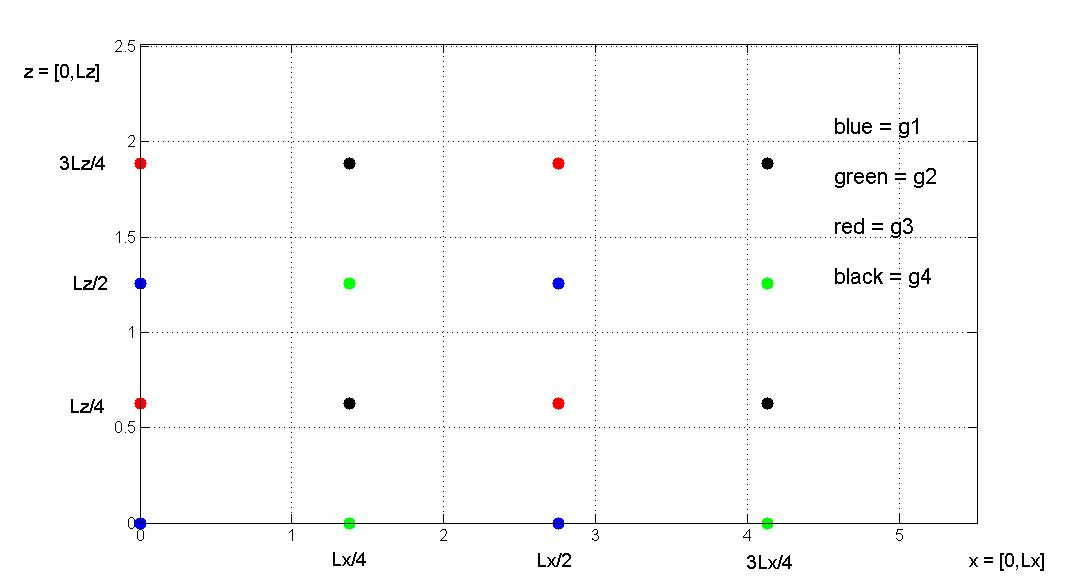
\includegraphics[width=1.2\textwidth]{stags7_26.jpg}
  \caption{
   Sets of possible \stagp s. If one of the $g$ symmetries is
   possessed, the velocity field will have \stagp s of the color
   corresponding to that $g$.
   }
  \label{eltonFig:stags7_26}
 \end{figure}



   \section{Equilibria \tEQsev\ and \tEQeight}
   \label{sect:EQ8}

\medskip\noindent {\bf  JFG July 26, 2008}:
n00bs.tex shows a couple equilibria in the HKW box with quarter-box
shifts. It's not too deep; you just take a solution with periodicity
$L_x$ and embed it in a box of length $2 L_x$. It would be better if
we could devise a good notation in which the symmetries of a solution
didn't depend on the box it was embedded in (i.e. were locked to the
periodicity of the solution rather than the box). Maybe it would be
sufficient to drop the $\tau_x^{1/2}$ shorthand in favor of the
longhand $\tau(\ell_x, 0)$.

I think that for a function of fundamental wave number $\alpha$
(Fourier expansion $\sum_n u_n \exp(i \alpha n x)$ with at least one
odd $u_n$ nonzero), the shifts in symmetry must be limited to $\ell_x =
\pi/\alpha$. Smaller shifts are not possible (for non-constant
functions) and bigger ones must be integer multiples, which are
equivalent to $\ell_x = \pi/\alpha$ due to periodicity. Right? I'll
put pencil to paper and check.

\medskip\noindent {\bf  JRE July 26, 2008 Question}:
   "There are equilibria with other symmetries
that fix $x,z$ phase but have other translations than the half-cell
shifts."

Other than EQ1 - EQ11? Could you tell me what these translations
are, or where to look? It could help to understand the nontrivial
\stagp s of EQ2.

\medskip\noindent {\bf  JFG July 21, 2008}:
A couple comments to things stretching back a few weeks: (1) Schmiegel
$I$ group is $\{1, s_3, \tau_z, s_3 \tau_z\}$ in our notation. (2)
Why are most of the equilibria symmetric in the $S$ symmetries? In a nutshell,
we know that EQBs 1-8 are symmetric in $S = \{1, s_1, s_2, s_3 = s_1
s_2\}$ because they satisfy those symmetries numerically. There is no
a priori reason that eqbs should be $S$-symmetric, other than $S$ symmetry
fixes $x,z$ phase and so rules out relative equilibria. But $s_3$ symmetry
alone does the same, and we have a few eqbs that have $s_3$ symmetry
but neither $s_1$ nor $s_2$ symmetry. There are equilibria with other symmetries
that fix $x,z$ phase but have other translations than the half-cell shifts.
In a rough sense, the half-cell shifts allow for the most gentle curvature
in the solutions, so these will generally have lower dissipation rates, be
more stable, and consequently more dynamically important than other shifts.

A bit of history will clarify. Nagata discovered the UB and LB EQBs in
1990 by continuing a known solution from Taylor-Couette flow to plane
Couette. He doesn't say anything about the symmetries, but Waleffe
calculated the same solutions a different way and noted that they
satisfy 'shift-rotate' and 'shift-reflect' symmetry (our $s_1$ and
$s_2$). We started our explorations of plane Couette dynamics around
those EQBs, noted that $S=\{1, s_1, s_2, s_3 = s_1 s_2\}$ is a group
and that the $S$-symmetric subspace was invariant under Navier-Stokes.
We focused our searches for new equilibria on this subspace, since it
fixes the $x,z$ phase of solutions and since the symmetry restriction
reduces the dimensionality of the eqbs' unstable manifolds. So we have
found $S$-symmetric eqbs primarily because we initiated our guesses
within that invariant subspace. However, the subspace is unstable, and
numerical simulations will creep away from it after a long time. Some
of our initial guesses had sufficient deviation from the $S$-symmetric
subspace that the Newton search was able to detect eqbs that lied
close to but were not actually within that subspace. That gave us EQBs
9, 10, and 11, which are $s_3$ symmetric but not $s_1$ or $s_2$.

We would probably do well to look for solutions with other symmetries. Where
that stands in terms of priorities, I'm not sure. It might be wise to listen
to Predrag (no, I'm not kidding) and factor out the continuous symmetries
beforehand, so that we don't have to conduct N different searches for N
different invariant subspaces.

\medskip\noindent {\bf  PC Aug 4, 2008}: I need to deconstruct the
$s_i$ notation for \refref{HGC08}.
The translation table for Elton's invariance group of
\tEQsev\ and \tEQeight\ is
\[
\{ s_1, \cdots, s_7 \} =
\{ \sigma_{z}\trHalf{x},
\sigma_{xy}\trHalf{xz},
\sigma_{xyz}\trHalf{z},,
\sigma_{z}\trHalf{z},
\sigma_{xyz}\trHalf{x}
\trHalf{xz},
\sigma_{xy}\}.
\] %ee{sj2sigtau}
% \nnu \\
% \label{shiftRot} \\
Using spanwise quarter-shift along $z$ we get rid of some half-shifts
\[
s_3 \to \sigma_{xyz}, s_1 \to \sigma_{z}\trHalf{xz},
s_4 \to \sigma_{z}, s_5 = \sigma_{xyz}\trHalf{xz},
\]
so a ``canonical'' form of the isotropy group is
\bea
A_{xz} &=& \{
e, \sigma_{xy}, \sigma_{z}, \sigma_{xyz},
\trHalf{xz}, \sigma_{xy}\trHalf{xz},
\sigma_{z}\trHalf{xz}, \sigma_{xyz}\trHalf{xz}
     \}
   \continue
   &=& \{e, \sigma_{xy}, \sigma_{z}, \sigma_{xyz}\}
        \times \{e,\trHalf{xz}\}
\,.
\label{tEQeightInv}
\eea
According to Halcrow doctrine, factor $\{e,\trHalf{xz}\}$ means
that the state lives on diamond 1/2 $[L_x,L_z]$ area, tiles the
cell twice.

   \medskip\noindent {\bf  JRE July 17, 2008}: We now have the
   remaining two symmetries to complete the group. JFG comment:
"The \tEQsev\ and \tEQeight\ are unique among the equilibria
discussed here in that they are also symmetric under $\tau_{xz}$ as
well as $s \in S$." Indeed, that is one of them,
$\tau(L_x/2,L_z/2)$. The other turns out to be $\sigma_2$. Defining
these to be $s_6 = \tau(L_x/2,L_z/2)$ and $s_7 = \sigma_2$ we have
that $S = \{e, s_1, s_2, s_3, s_4, s_5, s_6, s_7\}$ and, as PC
comments allude to, S is now a group of order 8, isomorphic to
$D_4$.

 \begin{align}
 &s_is_i = e \hspace{2 mm}\text{for each element of}\hspace{2 mm} S \\
 &s_1s_2 = s_3,\hspace{2 mm} s_1s_3 = s_2,\hspace{2 mm} s_1s_4 = s_6,\hspace{2 mm} s_1s_5 =
 s_7,\hspace{2 mm} s_1s_6 = s_4,\hspace{2 mm} s_1s_7 = s_5 \\
 &s_2s_3 = s_1,\hspace{2 mm} s_2s_4 = s_5,\hspace{2 mm} s_2s_5 = s_4,\hspace{2 mm} s_2s_6 =
 s_7,\hspace{2 mm} s_2s_7 = s_6 \\
 &s_3s_4 = s_7,\hspace{2 mm} s_3s_5 = s_6,\hspace{2 mm} s_3s_6 = s_5,\hspace{2 mm} s_3s_7 =
 s_4 \\
 &s_4s_5 = s_2,\hspace{2 mm} s_4s_6 = s_1,\hspace{2 mm} s_4s_7 = s_3 \\
 &s_5s_6 = s_3,\hspace{2 mm} s_5s_7 = s_1 \\
 &s_6s_7 = s_2 \\
  \end{align}



\medskip\noindent {\bf  PC July 16, 2008}:
Very nice!
The perspective view of \reffig{eltonFig:usquare_EQ8_1} is very interesting.
This volume-preserving flow (area preserving in Poincar\'e sections) probably
has invariant tori - you might be onto something there. Being quasiperiodic,
they would not be detected by your \eqva\ searching routines. Finding
a \stagp\ with purely imaginary eigenvalue would be a strong indication.
So far your eigenvalues are all over the place (their inverses set
dynamical time-scales, at least in neighborhoods if \stagp s), so
it is hard to tell.
Real part of \refeq{EQSP5eigs} seems small, though.



\medskip\noindent {\bf  JRE July 16, 2008}: \tEQsev\ and \tEQeight\ possess two
new symmetries that are not included in the subgroup $S$ from
\refsect{JHsec:4/28}. These are $s_4 = \tau(0,L_z/2) \, \sigma_1$
and $s_5 = s_4s_2$, where $s_2$ is the same as it was previously.
These new symmetries act on velocity fields as
\begin{align}
s_4 \, [u, v, w](x,y,z) &= [u, v, -w](x,\, y,\, -z+L_z/2) \nnu \\
s_2 \, [u, v, w](x,y,z) &= [-u, -v, w](-x+L_x/2,\,-y,\,z+L_z/2) \label{eqn:newgroup} \\
s_5 \, [u, v, w](x,y,z) &= [-u,-v,-w](-x+L_x/2,\, -y,\, -z) \nnu \,.
\end{align}
It can be checked that, similar to before, the set $ \{e, s_4, s_2,
s_5\}$ forms an Abelian group. It is not true, however, that the set
$ \{e, s_1, s_2, s_3, s_4, s_5\}$ which contains all of the
symmetries forms a group.

\medskip\noindent {\bf  PC July 16, 2008}:
$ \{e, s_1, s_2, s_3, s_4, s_5\}$ is probably a subset of elements of
a group of order 8. Presumably $D_4$, the product of four $D_1$ groups,
two for refections, and
two for spanwise, streamwise 1/2-cell translations,
if I remember correctly.
Keep multiplying, it should close. There might be \eqva\ hiding in
this invariant subspace.

Please check {\bf JFG May 23, 2008} discussion of Schmiegel's
symmetry groups, currently section 8.22 of Halcrow blog.
You might have run into a yet another symmetry subgroup,
like Schmiegel's $I$ group, but different. In halcrow/n00bsie\rf{HGC08}
JFG writes: ``\tEQsev\ and \tEQeight\ are $S$ symmetric (...).
 They appear to
be equivalent to the $\sigma$ solutions from \cite{Schmi99}, where they appear
to be the outer envelope in the $D$ versus $\Reynolds$ bifurcation diagram.
(...). The \tEQsev\ and \tEQeight\ are
unique among the \eqva\ discussed here in that they are also symmetric under
$\tau_{xz}$  as well as $s \in S$.''

\medskip\noindent {\bf  JRE July 16, 2008}:
 From \refeq{eqn:newgroup} we also see that
for \tEQsev\ and \tEQeight\ these symmetries imply that we will have
additional \stagp s at locations where $(x,y,z) = (-x+L_x/2,\, -y,\,
-z)$. This provides us with the 4 new \stagp s \bea
  \xSP{5} &=& (L_x/4,0,0) \continue
  \xSP{6} &=& (3L_x/4,0,0) \continue
  \xSP{7} &=& (L_x/4,0,L_z/2)  \\
  \xSP{8} &=& (3L_x/4,0,L_z/2) \nnu
 \,.
\eea
 Note that these \stagp s occur in pairs that are symmetric about
 the old \stagp s SP1-SP4, as they must by the discussion in
 \refsect{sect:stagpairs}. I actually came about this in the opposite order. A Newton search on
\tEQeight\ revealed that $(L_x/4,0,L_z/2)$ and $(3L_x/4,0,L_z/2)$
are \stagp s. From this one may deduce that symmetry $s_5$ must
hold, and it can then be checked that at any position the velocity
field is indeed invariant under $s_4$ and $s_5$. I have checked all
11 of the equilibrium velocity fields, and curiously only \tEQsev\
and \tEQeight\ are invariant under these additional symmetries.
Stability analysis of the new set for \tEQeight\ gives the
following.

 \tSP{5}: There is one real, positive eigenvalue
 and a complex pair with negative real part.
  \begin{align} &\eigExp[1] = 0.03109 \,,\quad \jEigvec[1] =
\begin{pmatrix}
             {0.85275} \cr
             {0.41774} \cr
             {-0.31355} \cr
   \end{pmatrix}
   \\
&\{ \eigExp[2],\eigExp[3]\}
  = \eigRe[2] \pm i \,\eigIm[2] =  -0.01555 \pm i\, 0.59385
   \label{EQSP5eigs}\\
&\jEigvec[2] =
\begin{pmatrix}
             {~0.24762} \cr
             {-0.31442} \cr
             {~0.69906} \cr
   \end{pmatrix}
    \,,\quad
\jEigvec[3] =
\begin{pmatrix}
             {-0.20793} \cr
             {~0.55489} \cr
             {~0} \cr
   \end{pmatrix}
\,.
\end{align}
 We have a 1D unstable manifold and a 2D in-spiral
stable manifold. All four of the new points have the same
eigenvalues. \tSP5 and \tSP8 have the same eigenvectors, as do \tSP6
and \tSP7 whose eigenvectors differ from \tSP5 only by the sign of
the third component for \jEigvec[1] and by the sign of the first and
second components for \jEigvec[2] and \jEigvec[3].

Another interesting although not necessarily useful result of
numerically searching for \stagp s is the figures produced by
plotting gridpoints where velocity squared is small. For a cutoff
value of $\mathbf{u}^{2}$ which is too large to be useful for
finding \stagp s we get a plot of points which has interesting and
intricate patterns. \reffig{eltonFig:usquare_EQ8_1} shows a 3D
perspective view of these points, and
\reffig{eltonFig:usquare_EQ8_2} and \reffig{eltonFig:usquare_EQ8_3}
show the projection of \reffig{eltonFig:usquare_EQ8_1} onto the $xz$
and $yz$ planes, respectively. Again, this is probably just more
visually amusing than useful but I was surprised to see the patterns
especially in \reffig{eltonFig:usquare_EQ8_2}. \\

\begin{figure}[!h]
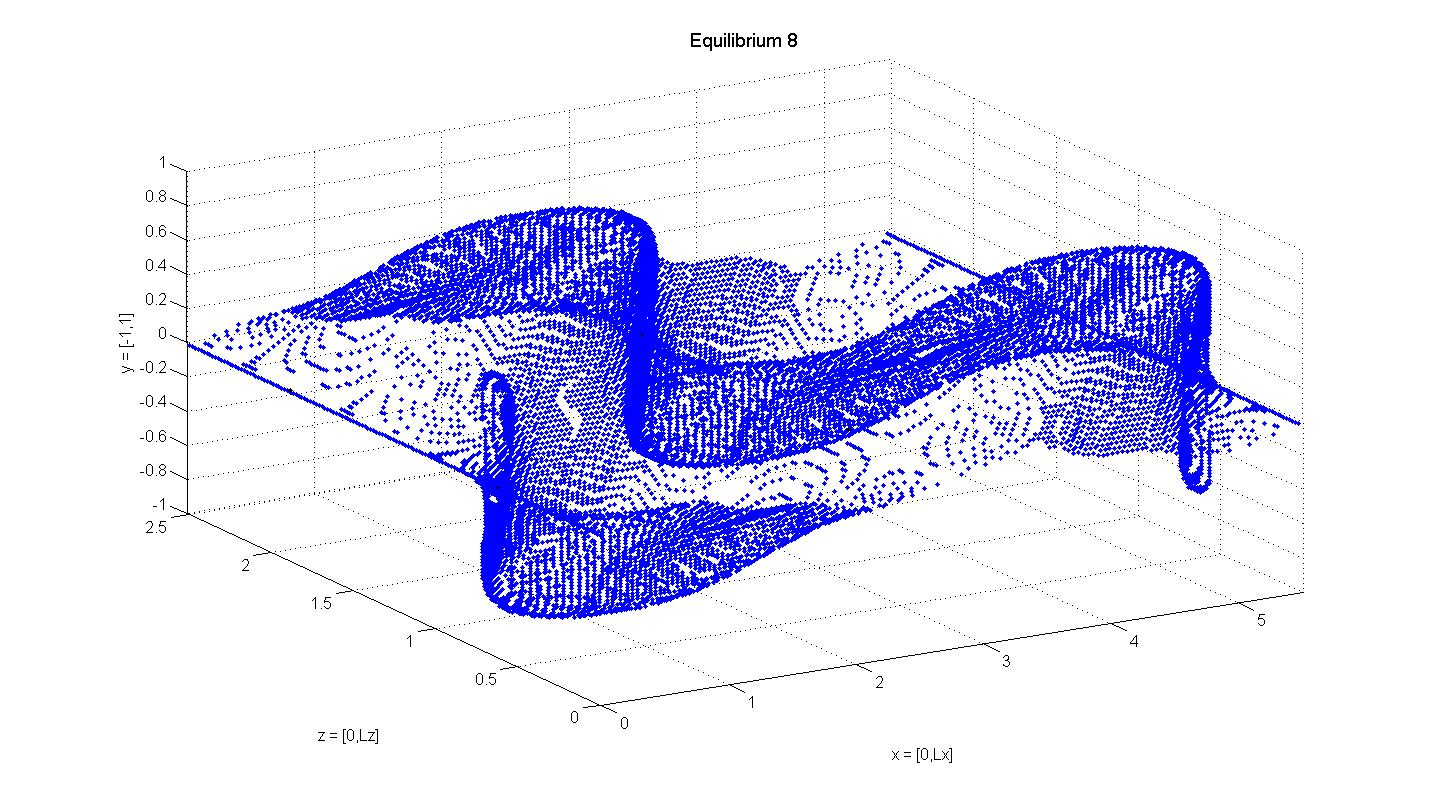
\includegraphics[width=1.4\textwidth]{usquare_EQ8_cute1.jpg}
  \caption{
   A plot of points whose value of velocity squared falls below an
   arbitrary cutoff of $5\times 10^{-7}$. Perspective view.
   }
  \label{eltonFig:usquare_EQ8_1}
 \end{figure}

 \begin{figure}[!h]
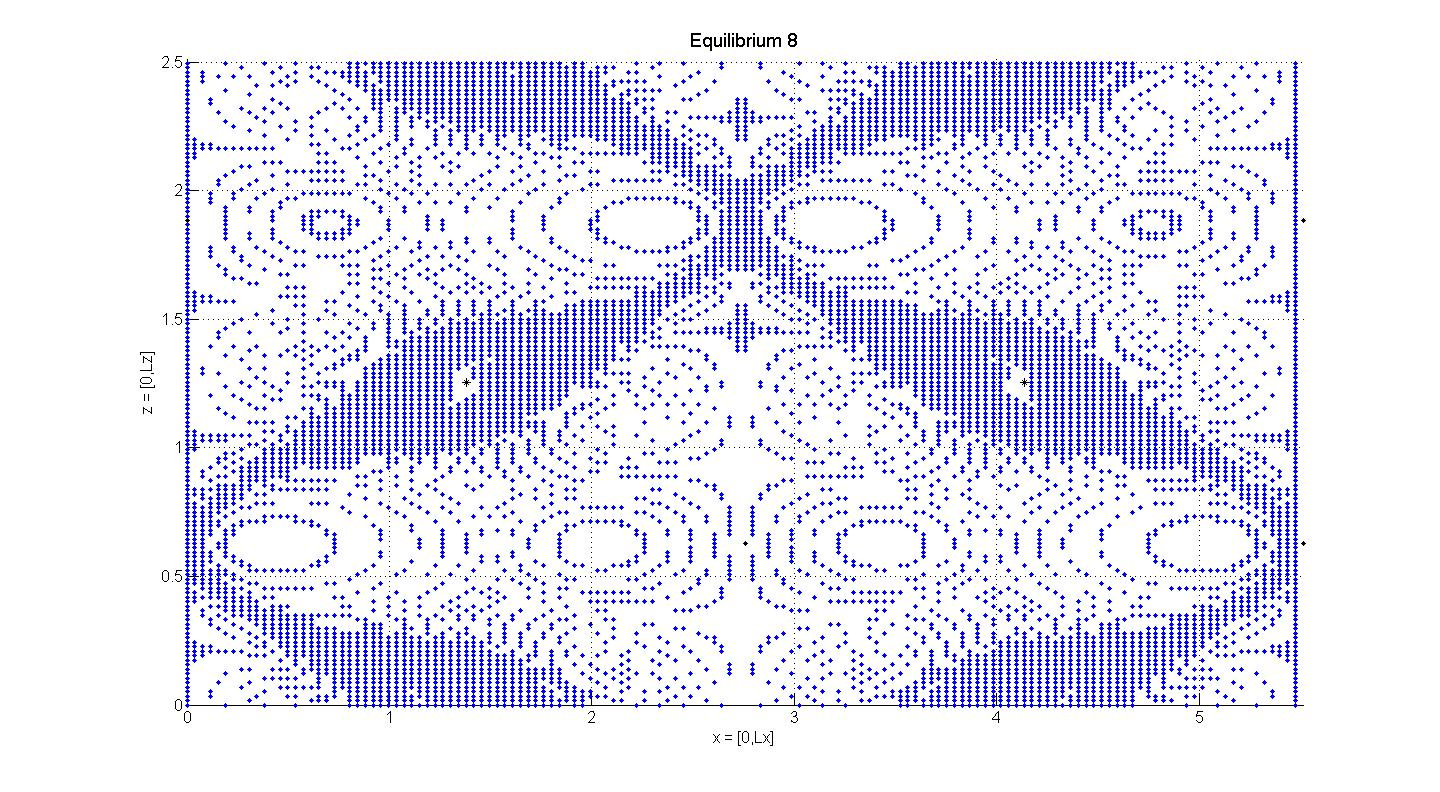
\includegraphics[width=1.4\textwidth]{usquare_EQ8_cute2.jpg}
  \caption{
   A plot of points whose value of velocity squared falls below an
   arbitrary cutoff of $5\times 10^{-7}$. Projection onto the $xz$
   plane.
   }
  \label{eltonFig:usquare_EQ8_2}
 \end{figure}

 \begin{figure}[!h]
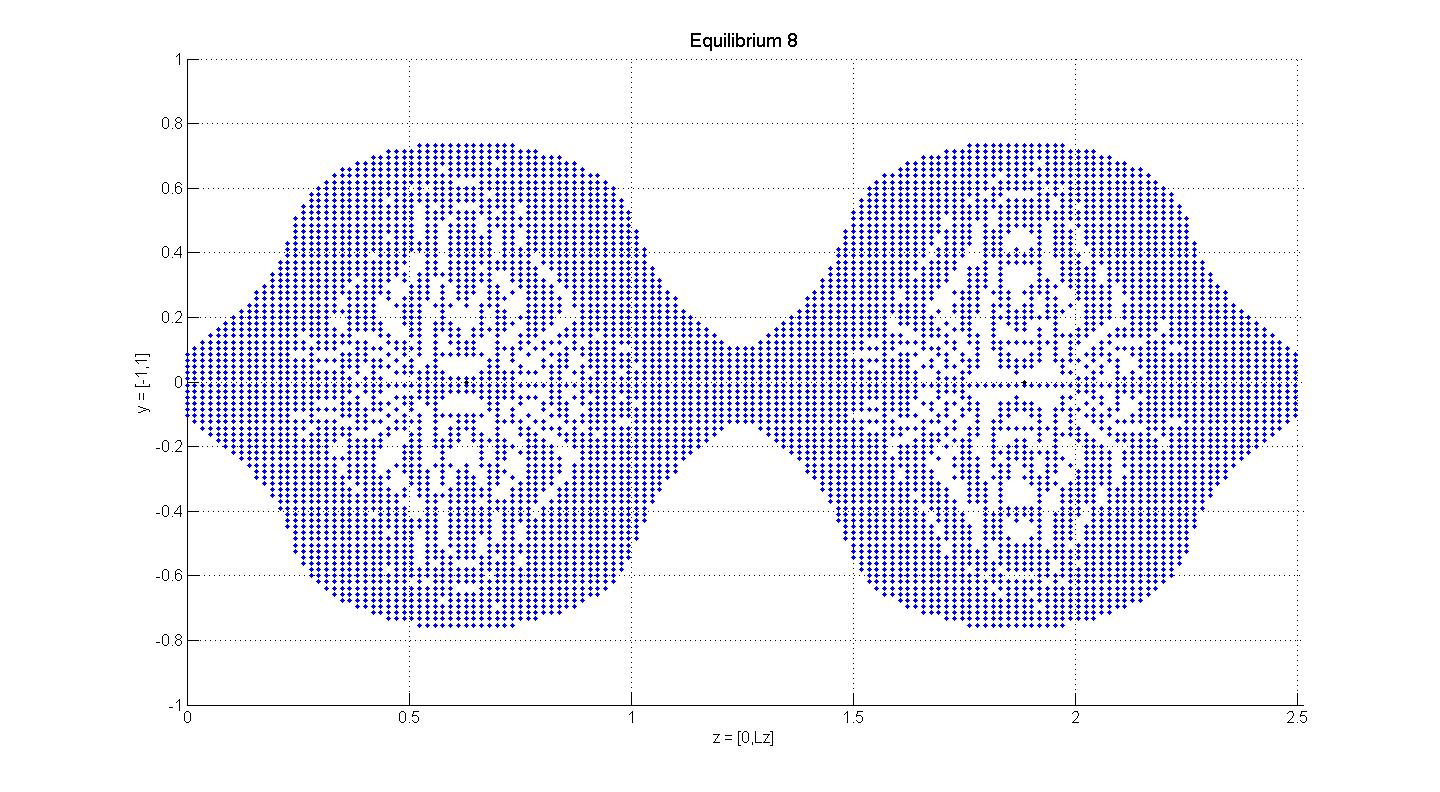
\includegraphics[width=1.4\textwidth]{usquare_EQ8_cute3.jpg}
  \caption{
   A plot of points whose value of velocity squared falls below an
   arbitrary cutoff of $5\times 10^{-7}$. Projection onto the $yz$
   plane.
   }
  \label{eltonFig:usquare_EQ8_3}
 \end{figure}


   \noindent {\bf  PC July 11, 2008}: Factorization of \tEQeight\
\tSP{1} and \tSP{1} stability eigenspaces is presumably due to symmetry
\refeq{S3project}; spanwise $z$ direction is $1D$ flow-invariant subspace at
the \stagp s. That ensures the simplicity of the \hec.

  \noindent {\bf  JRE August 12, 2008}: After going through the
  usual techniques for EQ7 it appears that it's features are
  largely resemblant of EQ8. We were already aware of the
  eight \stagp s, and the heteroclinic connection between SP1 and
  SP2 appears as well. The one qualitative difference I spot is
  that for SP1 in the plane perpendicular to the direction of the
  heteroclinic connection the eigenvalues are complex, whereas for
  EQ8 all three were real.

   \noindent {\bf  JRE July 9, 2008}:
 We will perform a similar analysis of \tEQeight\ and \tLB\ to that of the Upper
 Branch (\tUB). We start here with \tEQeight, which is a more turbulent
 flow with \Reynolds\ 270.

 Begin once again with a cleverly chosen grid of initial
 trajectories to get a feel for the significant structures in the
 flow (this time it was clever, last time it was lucky). The grid is
 in a plane at $x = L_{x}/2$. The result, after a short integration
 time, is shown in \reffig{eltonFig:EQ8_grid1}. This perspective
 view already shows us quite a bit of information. Once again we
 have symmetries abound, as expected. The points
 $(L_{x}/2,0,L_{z}/4)$ and $(L_{x}/2,0,3L_{z}/4)$ are \stagp s of this
 velocity field as well (as confirmed numerically). A
 shifted plot where the grid lies on the plane $x = 0$ reveals the
 same picture, rotated. This is to be expected (see
 \refsect{subsection:symmquest}
 below for discussion about this). Another interesting part of this
 plot is the four vortical structures on the left half. It may be
 that there are more \stagp s centered here, in any case they
 obviously contribute to the interesting dynamics. One final point
 of interest from this plot is the perfect line segment connecting
 the points that I was previously calling \tSP{1} and \tSP{2}. Note that
 because of the finite grid size the line segment does not originate
 right on \tSP{1}, however other more fine plots and rotational views (not shown) make it clear that this is so.
  This basically already implies a heteroclinic
 connection between these two \stagp s. To confirm this I have
 computed the eigenvalues and eigenvectors of the \velgradmat. For
 \tSP{1} (I realize we need a different naming convention), there is
 indeed a real, unstable eigenvector pointing along (0,0,1) and for
 \tSP{2} there is a real, stable eigenvector pointing along (0,0,1).
 This, together with the plot, essentially numerically proves the conjecture beyond reasonable
 doubt. The same result of course holds for the shifted pair at $x = 0$. The rest of the eigenvalues/eigenvectors are given
 below. It is interesting that for \tEQeight\ there is a heteroclinic connection which is a perfectly
 horizontal line connecting the pair of trivial \stagp s in the
 spanwise direction, whereas for \tUB\ the connection was some
 funny curve in the streamwise direction connected to a nontrivial
 \stagp.

\tEQeight, \tSP{1}: There are two real, positive eigenvalues
 and one real, negative eigenvalue.
    \PC{reordered eigenvalues by their magnitude}
\bea
\left(
    \eigExp[1],\eigExp[2],\eigExp[3]
\right) &=&
      (0.363557,0.227831,-0.591389)
\label{E8SP1} \\
\left(
    \jEigvec[1],\jEigvec[2],\jEigvec[3]
\right) &=&
\left(
    \begin{pmatrix}
             {0} \cr
             {0} \cr
             {1}
    \end{pmatrix} \,,
    \begin{pmatrix}
             {-0.733415} \cr
             {-0.679780} \cr
             {0}
    \end{pmatrix} \,,
    \begin{pmatrix}
             {0.991005} \cr
             {0.133824} \cr
             {0}
    \end{pmatrix}
\right) \,.
\nnu
\eea

\tEQeight, \tSP{2}: There are two real, positive eigenvalues
 and one real, negative eigenvalue.
\bea
\left(
    \eigExp[1],\eigExp[2],\eigExp[3]
\right) &=&
      (0.992857,0.255973,-1.248830)
\label{E8SP2} \\
\left(
    \jEigvec[1],\jEigvec[2],\jEigvec[3]
\right) &=&
\left(
    \begin{pmatrix}
             {~0.116961} \cr
             {-0.993136} \cr
             {0}
    \end{pmatrix} \,,
    \begin{pmatrix}
             {0.957795} \cr
             {0.287450} \cr
             {0}
    \end{pmatrix} \,,
    \begin{pmatrix}
             {0} \cr
             {0} \cr
             {1}
    \end{pmatrix}
\right) \,.
\nnu
\eea


   \begin{figure}[!h]
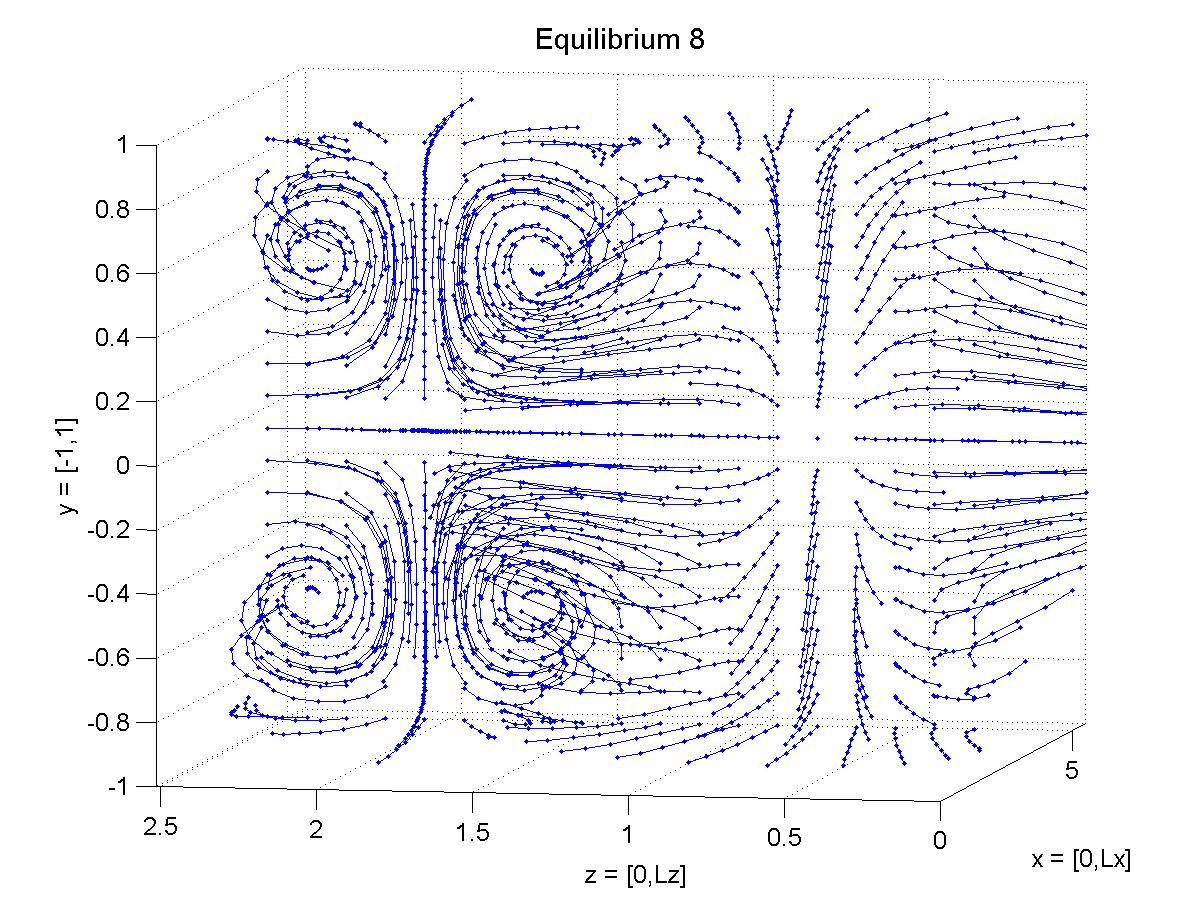
\includegraphics[width=1.4\textwidth]{EQ8_grid1.jpg}
  \caption{
   A grid of initial trajectories in the plane $x = L_{x}/2$
   integrated for short time.
   }
  \label{eltonFig:EQ8_grid1}
 \end{figure}


\subsection{Question on symmetries}
\label{subsection:symmquest}
  I have confirmed for myself that the
\NS\ equations are invariant for any symmetry in the group generated
by $\sigma_{1}, \sigma_{2}, \tau$. What I'm not clear on is the
following:
   In \refsect{JHsec:4/28} it is stated that
  "Most of the Eulerian \eqva\ that we know of so far
are invariant under the `shift-reflect' symmetry $s_1 =
\tau(L_x/2,0) \, \sigma_1$ and the `shift-rotate' symmetry $s_2 =
\tau(L_x/z,L_z/2) \, \sigma_2$.  These symmetries form a subgroup $S
= \{1, s_1, s_2, s_3\}$, $s_3 = s_1 s_2$, which is isomorphic to the
Abelian dihedral group $D_2$".
 First, I would like to ask how this
is known. Is there a theoretical argument for it, or is it simply
known empirically? From my numerical work it is certainly seen to be
true, ii is just not yet clear to me why, from first principles, that
this is so. Also, I should ask to confirm that it is known to be
true for EQ1 and EQ8, although I have already basically shown it for
EQ8.


\section{Proof that any new \stagp\ must have a partner lying on a line through an oldie (SP1-SP4), equidistant. }
 \label{sect:stagpairs}
 \noindent {\bf  JRE June 10, 2008}: This basically follows from the
 action of $s3 \in S$ on velocity fields (\refsect{JHsec:4/28}),
 \beq    s_3 \, [u, v, w](x,y,z) = [-u,-v,-w](-x,\, -y,\, -z+L_z/2)\nnu\, .
 \eeq
 If $(x_\tSP{},y_\tSP{},z_\tSP{})$ is a \stagp, $[u, v,
 w](x_\tSP{},y_\tSP{},z_\tSP{}) = [0,0,0]$, then
 \begin{align} s_3 \, [u, v, w](x_\tSP{},y_\tSP{},z_\tSP{}) &= [-u,-v,-w](-x_\tSP{},\, -y_\tSP{},\, -z_\tSP{}+L_z/2) \nnu\, \\
 &= [0,0,0](-x_\tSP{},\, -y_\tSP{},\, -z_\tSP{}+L_z/2) .
 \end{align}
 So $\xSP{'} =(-x_\tSP{},\, -y_\tSP{},\, -z_\tSP{}+L_z/2)$ is also a \stagp.

 \noindent We may parameterize a line passing through two points $x_{1},x_{2}$
 as
 \begin{align}
  x &= x_{1} + (x_{2} - x_{1})t \\
  y &= y_{1} + (y_{2} - y_{1})t \\
  z &= z_{1} + (z_{2} - z_{1})t \\
  t &\in (-\infty,\infty)
 \end{align}
 For the case above this becomes
 \begin{align}
  x &= x_\tSP{}(1-2t) \\
  y &= y_\tSP{}(1-2t) \\
  z &= z_\tSP{}(1-2t) + \frac{L_{z}}{2} t
 \end{align}
 When $t = 1/2$ this system returns $(x,y,z) = (0,0,L_{z}/4)$, showing
 that SP3 lies on the line between these two \stagp s and is halfway
 in between them.

 If we invoke the box periodicities: $x = x + L_{x}$, $z = z +
 L_{z}$, we can show that the pair of fixed points is symmetric
 about any of the other SP1-SP4. \\

 \noindent$\mathbf{x = x + L_{x}}$:

 \noindent$(x_\tSP{},y_\tSP{},z_\tSP{})$ a \stagp\ $\Rightarrow$
 $(-x_\tSP{}+L_{x},-y_\tSP{},z_\tSP{}+L_{z}/2)$ a \stagp.
 \begin{align}
  x &= x_\tSP{}(1-2t) + L_{x}t \\
  y &= y_\tSP{}(1-2t) \\
  z &= z_\tSP{}(1-2t) + \frac{L_{z}}{2} t
 \end{align}
 When $t = 1/2$ this returns $(x,y,z) = (L_{x}/2,0,L_{z}/4)$ so that the
 points lie symmetrically on a line passing through SP1. \\

 \noindent$\mathbf{z = z + L_{z}}$:

 \noindent$(x_\tSP{},y_\tSP{},z_\tSP{})$ a \stagp\ $\Rightarrow$
 $(-x_\tSP{},-y_\tSP{},z_\tSP{}+3L_{z}/2)$ a \stagp.
 \begin{align}
  x &= x_\tSP{}(1-2t) \\
  y &= y_\tSP{}(1-2t) \\
  z &= z_\tSP{}(1-2t) + 3\frac{L_{z}}{2} t
 \end{align}
 When $t = 1/2$ this returns $(x,y,z) = (0,0,3L_{z}/4)$ so that the
 points lie symmetrically on a line passing through SP4. And
 finally, \\

 \noindent$\mathbf{z = z + L_{z}},\mathbf{x = x + L_{x}}$:

 \noindent$(x_\tSP{},y_\tSP{},z_\tSP{})$ a \stagp\ $\Rightarrow$
 $(-x_\tSP{}+L_{x},-y_\tSP{},z_\tSP{}+3L_{z}/2)$ a \stagp.
 \begin{align}
  x &= x_\tSP{}(1-2t) + L_{x}t \\
  y &= y_\tSP{}(1-2t) \\
  z &= z_\tSP{}(1-2t) + 3\frac{L_{z}}{2} t
 \end{align}
 When $t = 1/2$ this returns $(x,y,z) = (L_{x}/2,0,3L_{z}/4)$ so that the
 points lie symmetrically on a line passing through SP2.

 This pairwise symmetric requirement for \stagp s is nice, but still
 there is the deeper question of, should any exist at all? I haven't
 been able to answer this yet, but a possible line of reasoning is
 the following: Any \stagp\ occurs at the intersection of the three
 surfaces $u = 0$, $v = 0$, $w = 0$. We know these three surfaces
 intersect at the four points SP1-SP4. Given that they are smooth, we might be able to come up with some
 kind of argument that shows that in fact these surfaces then
 $\emph{must}$ intersect somewhere else. It's a thought anyway.


\section{A colorful physical space portrait of the Upper Branch}
 \label{sect:colorportrait}
 \noindent {\bf  JRE June 04, 2008}: With a much faster interpolater
 and some improved plotting techniques, I have produced a picture
 of the dynamical behavior between our known \stagp s.

 First, in \reffig{eltonFig:stagps_label}, I have attempted to give
 a clear label of where these points lie within one periodic
 interval. SP1 through SP4 lie in the plane $y = 0$. SP5 and SP6 are
 symmetric about SP1. Note that a translation of SP6 would also lie in this box as well, situated
 below SP4, but I have chosen to omit it from this picture. At
 certain times it will be convenient to picture slightly different
 translations of these points than as they appear in
 \reffig{eltonFig:stagps_label}.

 The interesting dynamics and connections between the different \stagp s occur
 along the $x$ direction. To understand what is happening one needs
 to look only at a subset of these \stagp s that lies in the right or left half of the box, that
 is, in the interval $[0,L_{z}/2]$ or the interval $[L_{z}/2,L_{z}]$. I have chosen
 to give results for the points lying in the interval $[0,L_{z}/2]$. In
 the $x$ direction the most convenient interval is not actually
 $[0,L_{x}]$. I have chosen to look at the \stagp s in the open interval
 $(-L_{x}/2,L_{x})$, open so as to ignore the repeated translations on the boundary. Thus the domain of investigation is
 \beq \Omega = (-L_{x}/2,L_{x}) \times [-1,1] \times [0,L_{z}/2]
 \eeq
 Within this domain there are four \stagp s. They are SP1, SP3, SP5, and
 SP6.
 In \reffig{eltonFig:stagps_label2} I show these four points in $\Omega$. Note that SP6 is a
 translated version from the way it was viewed in
 \reffig{eltonFig:stagps_label}. The reason for this will soon be
 clear. \\

 I will start by discussing the most interesting result, the
 heteroclinic connections between SP5 and SP3, and similarly between SP6 and
 SP3. The picture is \reffig{eltonFig:hetero1}. These surfaces have
 kind of an eerie beauty. The red curves are the 1D unstable manifolds
 of SP5 and SP6, or equivalently the stable manifold of SP3. Their thick appearance
 is simply so that they can be seen within the blue surface. They are actually just a single trajectory. The
 blue surface, the unstable manifold of SP3, is found in the following way. A large number of initial
 conditions very close to SP3 (in the plane of it's unstable eigenvectors) are evolved forward in
 time. Because the integration always breaks down as these trajectories
 get near to SP5 and SP6, in practice I also plot the stable
 manifolds of SP5 and SP6 and connect them with the unstable
 manifold of SP3 in the middle region, where they are both accurate.

 We now bring SP1 into the picture. SP1 has a 2D unstable manifold
 and a 1D stable manifold. The result of all of these manifolds
 plotted together is \reffig{eltonFig:hetero2}. The relation of the
 stable manifold (yellow curve) and unstable manifold (green surface) of SP1
 to the blue surface is quite interesting. These trajectories
 tightly hug the blue surface as they spiral around it.

 One merely translates the image in \reffig{eltonFig:hetero2} in the
 $x$ direction by an amount $L_{x}$ to give a complete picture in
 any periodic cell. The same picture will also occur symmetrically
 (translated by $L_{x}/2$ and $L_{z}/2$) in the left half of the
 box.




 \begin{figure}[!h]
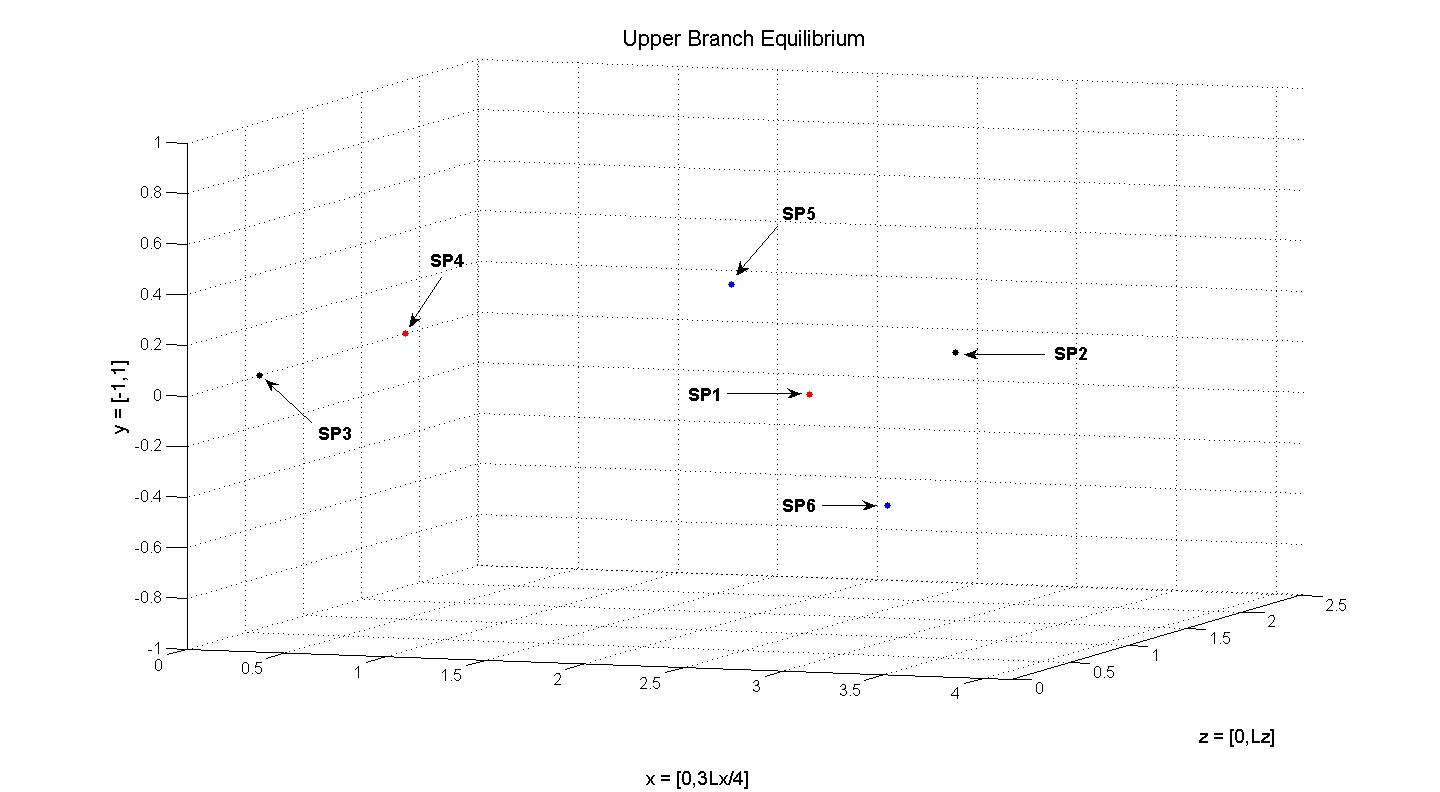
\includegraphics[width=1.5\textwidth]{stagps.jpg}
  \caption{
   The 6 known unique \stagp s within one periodic box, SP1 through
   SP6. The pair SP1 and SP4 are related through a symmetry, and
   similarly for the pairs SP2 with SP3, and SP5 with SP6.
   }
  \label{eltonFig:stagps_label}
 \end{figure}

 \begin{figure}[!h]
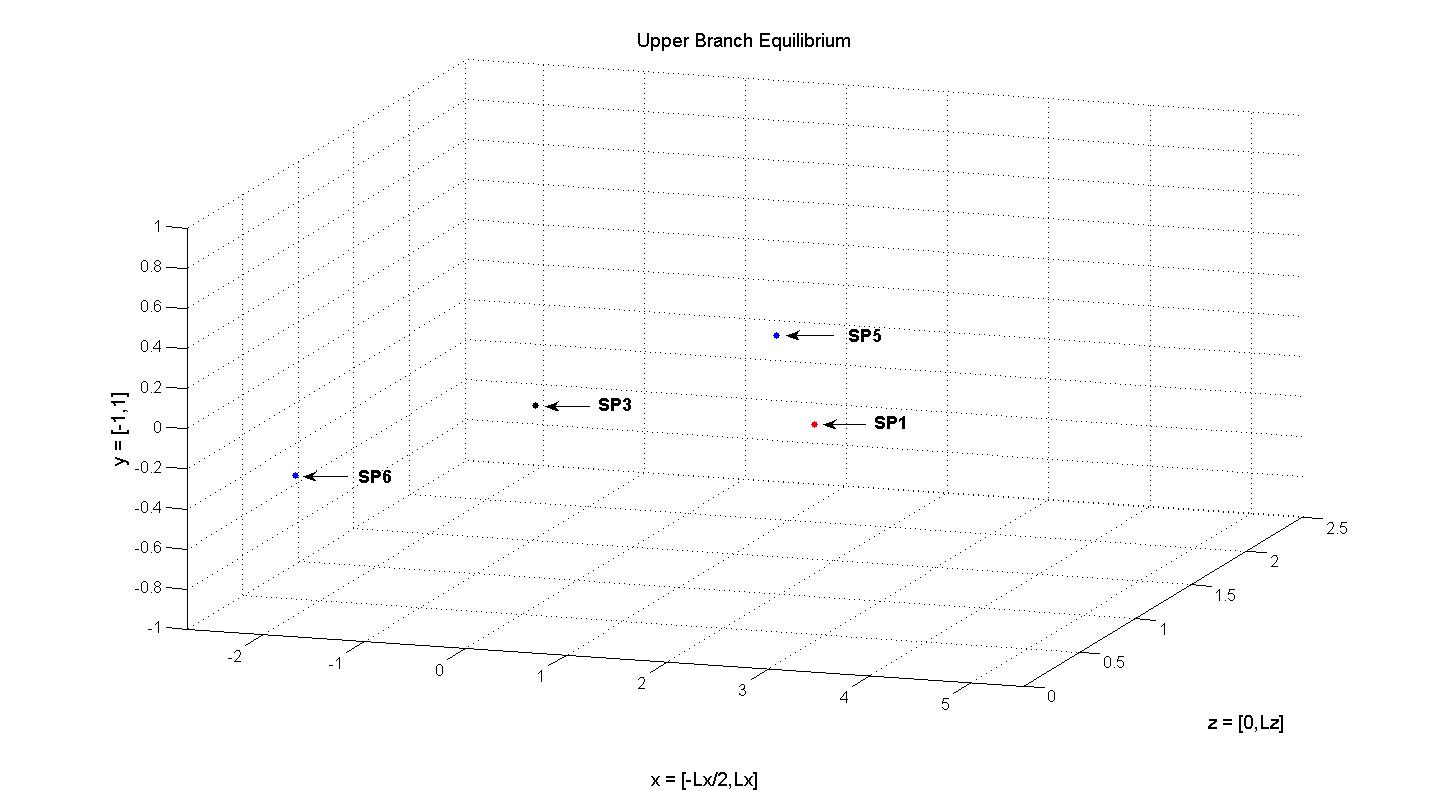
\includegraphics[width=1.3\textwidth]{stagps2.jpg}
  \caption{
   The 4 \stagp s that occur within the domain $\Omega$.
   }
  \label{eltonFig:stagps_label2}
 \end{figure}

 \begin{figure}[!h]
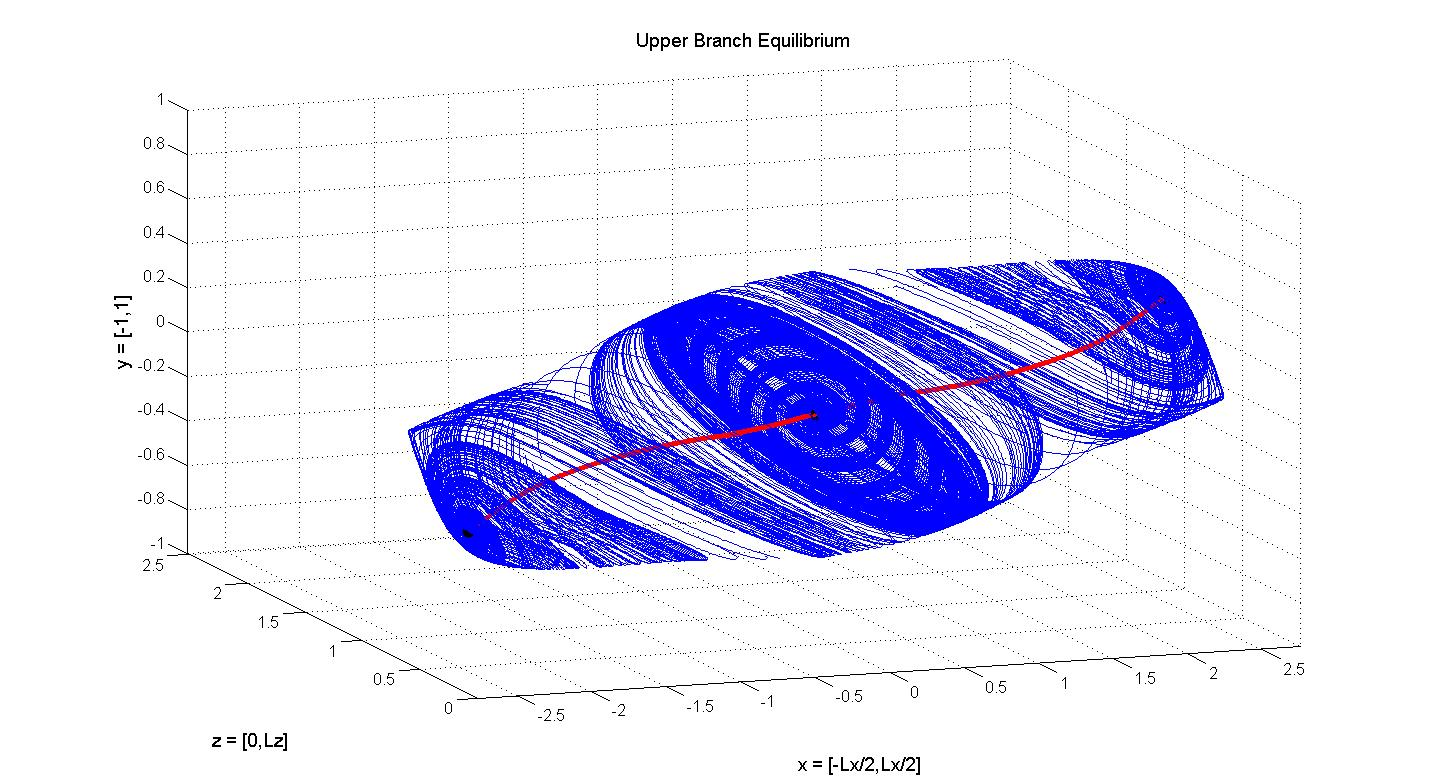
\includegraphics[width=1.3\textwidth]{man14_june3.jpg}
  \caption{
   Heteroclinic pairs.
   }
  \label{eltonFig:hetero1}
 \end{figure}

 \begin{figure}[!h]
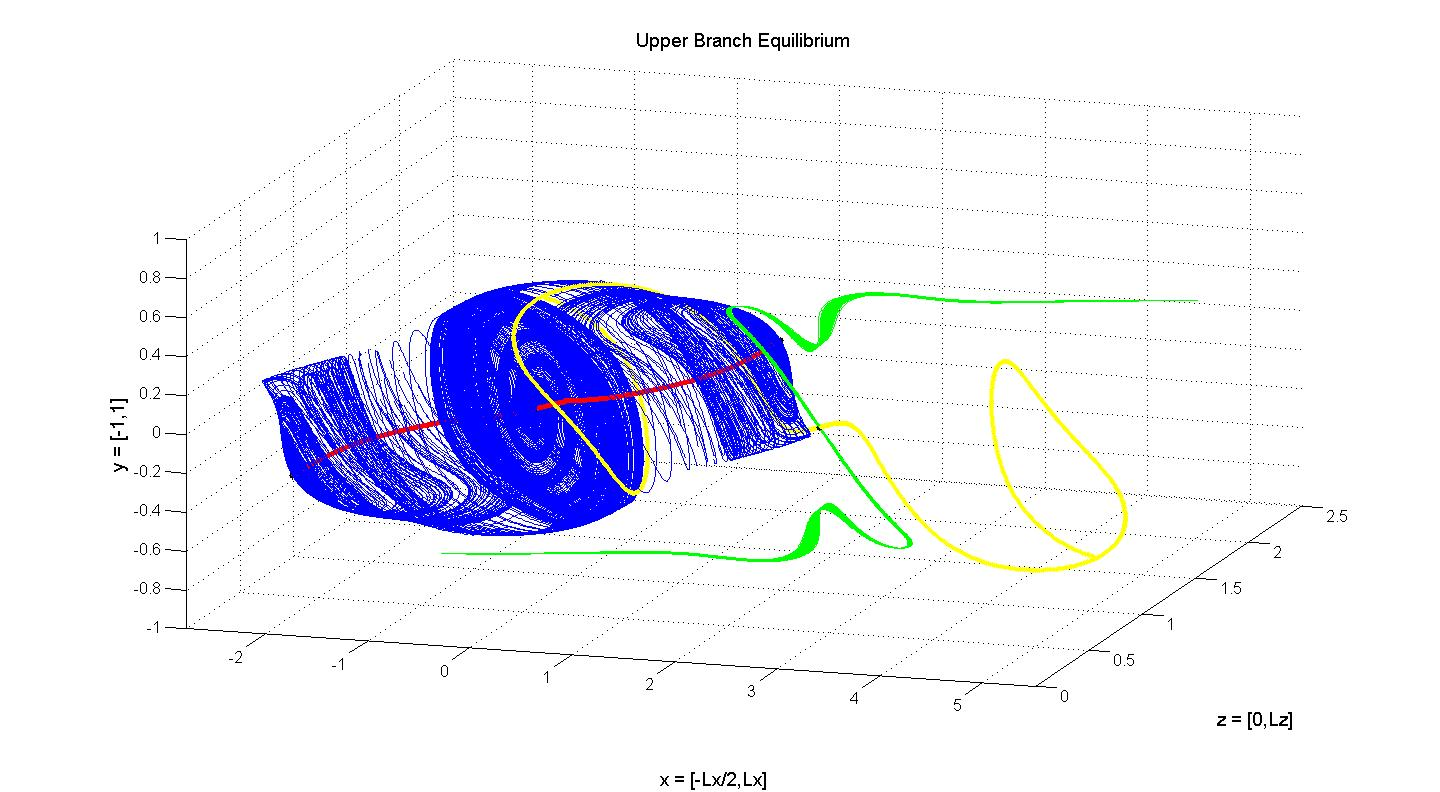
\includegraphics[width=1.3\textwidth]{june4_fig7.jpg}
  \caption{
   Full physical space relations between the \stagp s.
   }
  \label{eltonFig:hetero2}
 \end{figure}

\section{The \NS\ equations}
 \label{sect:NavierStokes}
 \noindent {\bf  JRE May 27, 2008}: The underlying equations
that govern the motion of \pCf\ are of course the \NS\ equations,
along with boundary conditions. The boundary conditions in the $x$
and $z$ directions are periodic,
 $ \bu(x, y, z) = \bu(x+L_x, y, z) =
\bu(x, y, z + L_z) $.
 In the $y$ direction,
 $\bu = (1,0,0)$ at $\bx = (0,1,0)$ and $\bu = (-1,0,0)$ at $\bx =
 (0,-1,0)$.

 The fluid is taken to be incompressible, so in this case the
 \NS\ equations are
 \beq
 \frac{\partial \bu}{\partial t} + (\bu \cdot \nabla)\bu = -\nabla p + \nu \nabla^{2} \bu
    \,,\qquad
\nabla \cdot \bu  = 0 \,. \label{eqn:NavierStokes} \eeq As far as I
know these are all of the conditions and assumptions that are made.
I would first like to confirm that this is correct, that
\refeq{eqn:NavierStokes} is the exact form of the \NS\ equations
that are being used for \pCf.

The starting point for everything that I have been doing so far is
to load the spectral coefficients,
$\mathbf{\hat{u}}_{m_{x},m_{y},m_{z}}$, from
\refeq{eqn:spectralsum}. From my perspective these coefficients are
kind of a magical data set that allows me to correctly compute
velocities, but of course I know they came from a DNS integration of
\refeq{eqn:NavierStokes}, namely through Channelflow.

For the Upper Branch equilibrium that I have been working with,
\refeq{eqn:NavierStokes} simplifies to \beq
 (\bu \cdot \nabla)\bu = -\nabla p + \nu \nabla^{2} \bu
    \,,\qquad \label{eqn:NavierStokes2} \eeq
 and the only other thing I know
about it is that $\Reynolds = 400$. I would prefer to know the exact
value of $\nu$ since it is the fundamental parameter in
\refeq{eqn:NavierStokes2}. Since \beq Re = \frac{\overline{u}L}{\nu}
\eeq where $\overline{u}$ is the average fluid velocity and $L$ is
the characteristic length, this amounts to asking what values are
taken for $\overline{u}$ and $L$? Or maybe someone already knows and
can tell me what $\nu$ is for this particular box at $\Reynolds =
400$. Interestingly, since I can compute \bu, $\nabla$\bu, and
$\nabla^{2}$\bu, as a crosscheck I could compute $\nu$ directly by
taking the curl of both sides of \refeq{eqn:NavierStokes2}. \\

At a \stagp\ of an equilibrium velocity field the \NS\ equations
\refeq{eqn:NavierStokes2} simplify further. At a point where $\bu =
0$, it is certainly true that
 \beq
  \nu \nabla^{2}\bu = - \nabla p,
    \label{eqn:NavierStokes3} \eeq
 and I think that this is probably a sufficient condition to specify a \stagp, for the following reason.

 When $(\bu \cdot \nabla)\bu$ is written out in component form we
 see that it is the vector
 \beq
 \begin{pmatrix}
             {u \frac{\partial u}{\partial x} +  v \frac{\partial u}{\partial y} + w \frac{\partial u}{\partial z}} \cr
             {u \frac{\partial v}{\partial x} +  v \frac{\partial v}{\partial y} + w \frac{\partial v}{\partial z}} \cr
             {u \frac{\partial w}{\partial x} +  v \frac{\partial w}{\partial y} + w \frac{\partial w}{\partial z}} \cr
   \end{pmatrix} =
   \begin{pmatrix}
             {\frac{\partial u}{\partial x}} &  {\frac{\partial u}{\partial y}} &  {\frac{\partial u}{\partial z}} \cr
             {\frac{\partial v}{\partial x}} &  {\frac{\partial v}{\partial y}} &  {\frac{\partial v}{\partial z}} \cr
             {\frac{\partial w}{\partial x}} &  {\frac{\partial w}{\partial y}} &  {\frac{\partial w}{\partial z}} \cr
   \end{pmatrix}
   \begin{pmatrix}
             {u} \cr
             {v} \cr
             {w} \cr
   \end{pmatrix} = A \bu
 \eeq
where $A$ is the \velgradmat. So if \refeq{eqn:NavierStokes3} holds
then $A \bu = 0$ and this implies we are at a \stagp\ unless the
nullspace of $A$ is nontrivial. This can only happen if the three
velocity gradients in $A$ are co-planar. This seems unlikely, and
there may be a physical reason that proves it can't ever happen. So
that's why I say I think \refeq{eqn:NavierStokes3} is a sufficient
condition for specifying a \stagp. It's simplified form may give
insight into solutions or symmetries for \stagp s. \\

 \noindent {\bf  JFG May 29, 2008}: In most of our work (and in channelflow) $\bu$
represents the {\em difference} from the laminar flow. I'll get to that in a minute,
but first I'll do the nondimensionalization to address the $\nu$ vs $Re$ issue.
Start with Navier-Stokes on the total fluid velocity field $\butot$
\beq
    \frac{\partial \butot}{\partial t}
    + \butot \cdot \bnabla \butot
=
    - \bnabla p
    +  \nu \lapl \butot \,, \quad \nabla \cdot \butot = 0
\ee{NavStokesRaw}
and boundary conditions $\butot = \pm U$ at $y = \pm L$. Rescale
variables: $y \rightarrow y/L$, (same for $x,z$), $u \rightarrow u/U$,
$t \rightarrow (U/L) \, t$, and $p  \rightarrow U^2 p$. That gives
\beq
    \frac{\partial \butot}{\partial t}
    + \butot \cdot \bnabla \butot
=
    - \bnabla p
    +  \frac{1}{Re} \lapl \butot \,, \quad \nabla \cdot \butot = 0,
\ee{NavStokesNondim} where $Re = UL/\nu$, and boundary conditions
$\butot = \pm 1\hat{\bf x}$ at $y = \pm 1$. This is the
nondimensionalized Navier-Stokes equation. You can think of the
nondimensionalized equations as having length scale $L=1$, velocity
scale $U=1$, and viscosity $\nu = 1/Re$, or better, the
nondimensional parameter $1/Re$ replacing viscosity.

Now break up the total velocity field into two components: $\butot =
y \hat{\bf x} + \bu$. Here $y \hat{\bf x}$ is the laminar velocity
field and $\bu$ is the difference between the total velocity and
laminar. Substitute $y \hat{\bf x} + \bu$ for $\butot$ in the
nondimensionalized Navier-Stokes equations to get

\beq
    \frac{\partial \bu}{\partial t}
    + y  \frac{\partial \bu}{\partial x}
    + v \, \hat{\bf x}
    + \bu \cdot \bnabla \bu
=
    - \bnabla p
    + \frac{1}{\Reynolds}
        \lapl \bu  \,, \quad \nabla \cdot \bu = 0
\, \
\ee{NavStokesDev}
and boundary conditions $\bu = 0 $ at $y \pm 1$.

The equilibrium fields such as $\tUB$ satisfy \refeq{NavStokesDev}.
 \JRE{Just to be completely clear, should we say the equilibrium fields such as $\tUB$ satisfy
 \refeq{NavStokesDev}, but with the $\frac{\partial \bu}{\partial
 t}$ term set to 0?}
  This equation is a little more complicated than
\refeq{NavStokesNondim}, but having Dirichlet boundary conditions on
$\bu$ makes analysis much easier, since the set of allowable $\bu$
form a vector space. The set of allowable $\butot$ doesn't, since
the sum of two allowable $\butot$ generally does not satisfy the
boundary condition $\butot = \pm 1$ at $y\pm 1$. By ``allowable'' I
mean those fields that satisfy incompressibility and boundary
conditions.

So, in a nutshell, (1) the equilibrium fields satisfy \refeq{NavStokesDev}, and
(2) you don't need $\nu$, you need $1/Re$.

Ok, that is just an explanation of our conventions, so that we're
all on the same page. Your larger issues stand, keeping in mind that
they apply to what we call $\butot$. But note how these issues play
out for the laminar solution. For $\butot = y \hat{\bf x}$, each of
the terms $1/Re \, \lapl \butot$, $\grad p$, and $\butot \cdot \grad
\butot$ is identically zero throughout the flow domain (in fact we
obtain $\grad p = 0$ from the other two identities.) But stagnation
points are limited to the plane $y=0$. So there are situations in
which the null space of $\butot \cdot \grad$ is nontrivial, and
$1/Re \, \lapl \butot = - \grad p$, does not imply stagnation. \\

 \noindent {\bf  JRE May 29, 2008}:
 Laminar example is a nice proof that it can in fact happen that
 $1/Re \, \lapl \butot = - \grad p$ does not imply stagnation, in this
 case because two of the velocity gradients in $A$ are identically
 zero. It still seems that in general for a typical velocity field
 there is no reason to expect that the three velocity gradients
 would lie in the same plane, so maybe we could say that
 $1/Re \, \lapl \butot = - \grad p$ implies stagnation, almost
 always?

\section{New \stagp s}
\label{sec:newstagps}

\noindent {\bf  JRE May 23, 2008}: Starting from the gridpoint value
\refeq{eqn:newsp} with smallest velocity in the suspicious region,
$\bx_{0} =(2.33476, 0.40952, 0.64577)$, and its reflection through
\xSP{1}, $\bx_{0}' =2 \xSP{1} - \bx_{0}$, the Newton iteration
 \beq
 \bx_{k+1} = \bx_{k} -
          {\Mvar}^{-1}(\bx_{k}) \, \bu(\bx_{k})
 \eeq
%  where $\Mvar$ is the \velgradmat.
converged rapidly to the new pair of \stagp s, accurate to
$\approx 10^{-16}$:
\PC{experimenting with upper case vs lower case for \tSPone. Will
settle on preferred notation later.}
\begin{align}
&\xSP{5} =(2.35105561774981,0.42293662349708,0.65200166068573)
\\
&\xSP{6}=(3.16051044117966,-0.42293662349708,0.60463540075018)
\label{eqn:newspNewt}
\,.
\end{align}
%         = [5.51156605892946182182,2,2.51327412287183459075]
We see the
 symmetry in the $y$-component of this pair, as was expected looking
 at \reffig{eltonFig:fine_usquare}.
These points are
 symmetric about the point $\tSP{1}$ in all three dimensions,
 \beq
    (\xSP{5} + \xSP{6})/2 = \xSP{1}
 \,.
 \eeq
It would
 be nice if we could think of a symmetry argument for their
 existence. However,
 unlike \refeq{s3lagrange} their components have no rational
 relation to $L_x$, $L_z$,
 so these are nontrivial \stagp s.

 \Stagp s \tSP{5}, \tSP{6}: There is one real, positive eigenvalue
 and a complex pair with negative real part.
 \PC{always write eigenvectors. I replaced these:
     \\
     $\jEigvec[2] =
\begin{pmatrix}
             {0.5226203 - 0.3779843i } \cr
             {-0.6703938} \cr
             {0.2065610 + 0.3031510i} \cr
   \end{pmatrix}
    \,,\quad
\jEigvec[3] =
\begin{pmatrix}
             {0.5226203 + 0.3779843i } \cr
             {-0.6703938} \cr
             {0.2065610 - 0.3031510i} \cr
   \end{pmatrix}
\,.
     $
     }
  \begin{align} &\eigExp[1] = 0.1453207 \,,\quad \jEigvec[1] =
\begin{pmatrix}
             {0.9307982} \cr
             {0.3502306} \cr
             {0.1046576} \cr
   \end{pmatrix}
   \\
&\{ \eigExp[2],\eigExp[3]\}
  = \eigRe[2] \pm i \,\eigIm[2] =  -0.0726603 \pm i\, 0.3733478
   \nnu\\
&\jEigvec[2] =
\begin{pmatrix}
             {~0.5226203} \cr
             {-0.6703938} \cr
             {~0.2065610} \cr
   \end{pmatrix}
    \,,\quad
\jEigvec[3] =
\begin{pmatrix}
             {~0.3779843} \cr
             {~
             0} \cr
             {- 0.3031510} \cr
   \end{pmatrix}
\,.
\end{align}
The \velgradmat\ is
\beq
   {\Mvar} =
   \begin{pmatrix}
   {0.0225166} &  {0.0985763} &{0.7623083} \cr
   {0.1714566} &   {-0.1275193} & {-0.6118476} \cr
   {-0.0615378}  &   {0.1755954}  & {0.1050028} \cr
            \end{pmatrix}
\,.
\eeq
We have this time a 1D unstable manifold and a 2D in-spiral stable
manifold.

   I have been labeling \stagp s to include all of the points which are
   inside a single periodic cell. However even within this cell
   there is a redundancy in labeling all of these points as
   distinct. There are really $\emph{three}$ distinct \stagp s in the fundamental domain and
   the rest result from invariance under $\bf{S}$ and should really be quotiented out.
   The dynamics between these three \stagp s and there translates is
   quite interesting. I began discussing possible heteroclinic
   connections in \refsect{sec:possibleconnect},
   and looking at \reffig{eltonFig:hetero54} it is
   now strongly suggestive that there exists a $\tSP{5} \to \tSP{4}$ \hec.
   The red curve is the stable manifold of $\tSP{4}$. The blue
   curve is the unstable manifold of the new $\tSP{5}$.
   I suspect that with a perfect integration these are
   one in the same.

   A complete phase space portrait (ignoring periodic orbits for
   the moment) should be coming soon. It looks like we have all of
   the \stagp s, and short of some numerical difficulties with
   plotting the stable and unstable manifolds we have a pretty good
   understanding of the interesting heteroclinic m\'enage \`a trois that is
   occurring between our three distinct \stagp s.
   \PC{In all figures: can you add a subroutine that plots all \stagp s,
       labeled}

\begin{figure}[!h]
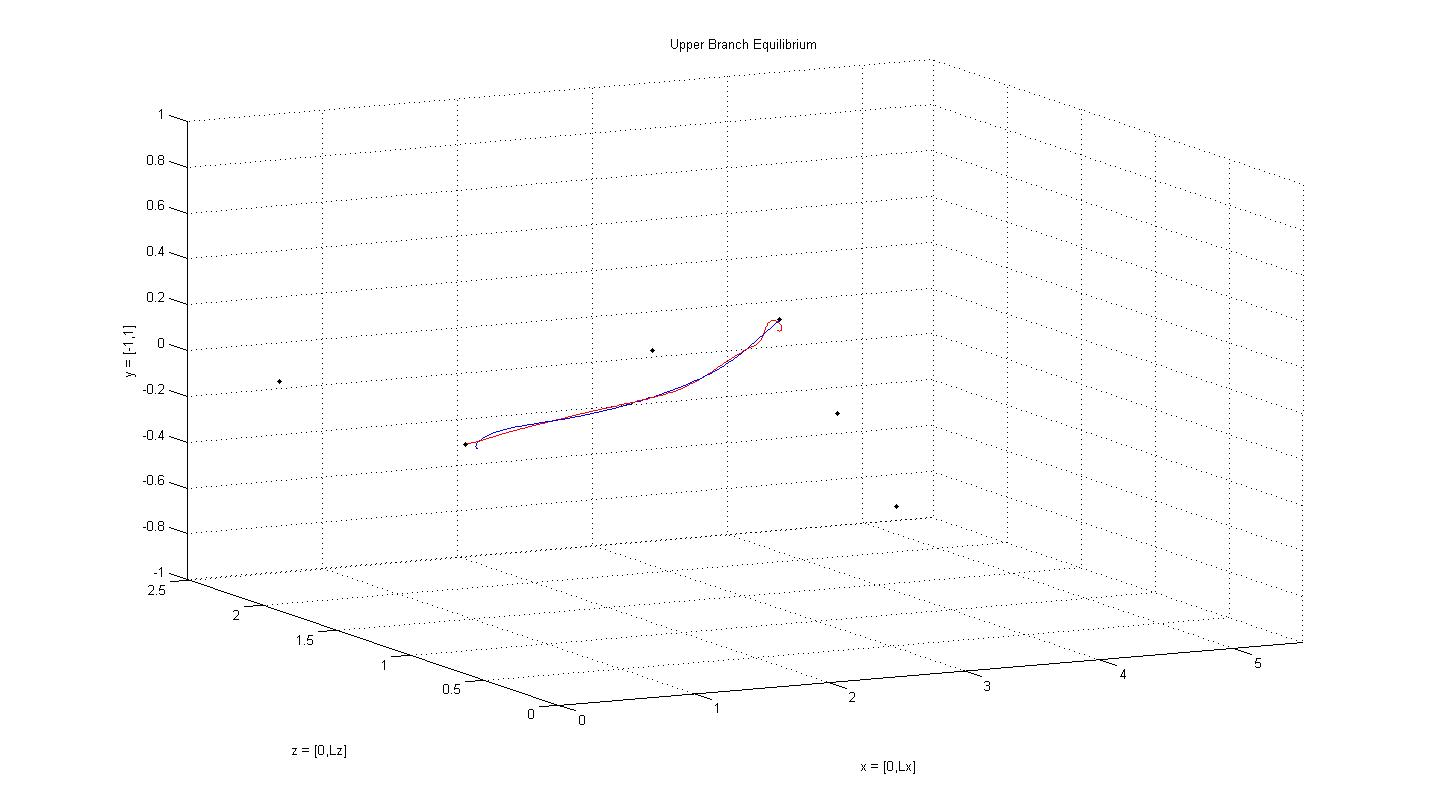
\includegraphics[width=1.3\textwidth]{hetero54.jpg}
  \caption{
   Stable manifold of $\tSP{4}$ (red curve) and unstable manifold of $\tSP{5}$ (blue curve).
   These are presumably the same and form a $\tSP{5} \to \tSP{4}$ \hec.
   }
  \label{eltonFig:hetero54}
 \end{figure}


\section{Possible \hec s and evidence of a new
pair of \stagp s}
\label{sec:possibleconnect}

\noindent {\bf  JRE May 21, 2008}:
 Of the four known \stagp s it appears that there may be a
 \hec\ between the two pairs of qualitatively different
 points.
% From now on it will be convenient to label the \stagp s
% \refeq{s3lagrange} as follows:
%\bea
%  \xSP{1} &=& (L_x/2,0,L_z/4) \continue
%  \xSP{2} &=& (L_x/2,0,3L_z/4) \continue
%  \xSP{3} &=& (0,0,L_z/4) \label{s3lagrange2} \\
%  \xSP{4} &=& (0,0,3L_z/4) \nnu
% \,.
%\eea
  \begin{figure}[!h]
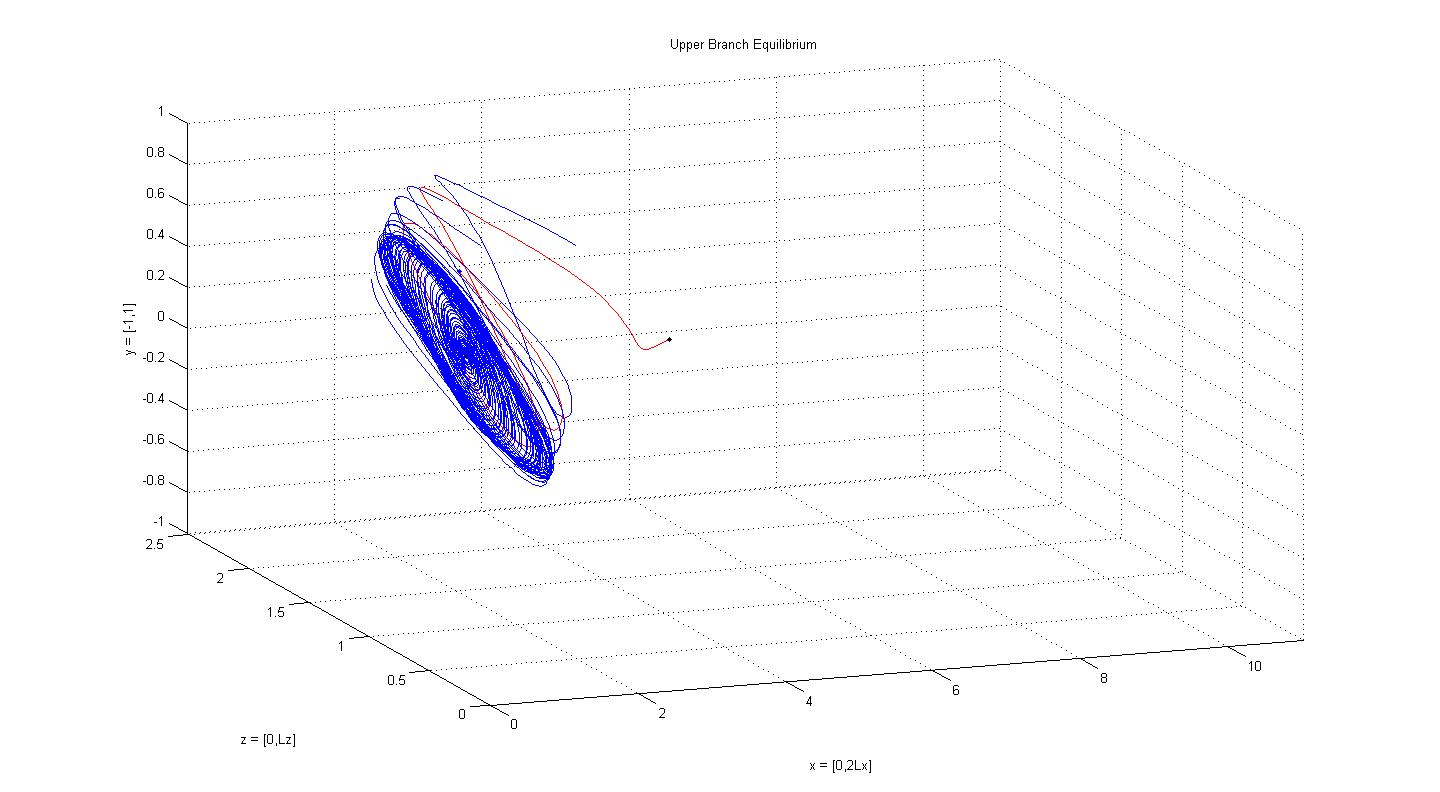
\includegraphics[width=1.3\textwidth]{almost_hetero24.jpg}
  \caption{
   Stable manifold of $\tSP{4}$ (red curve)
   and unstable manifold of $\tSP{2}$ (blue surface)}
  \label{eltonFig:almost_hetero24}
 \end{figure}
\begin{figure}[!h]
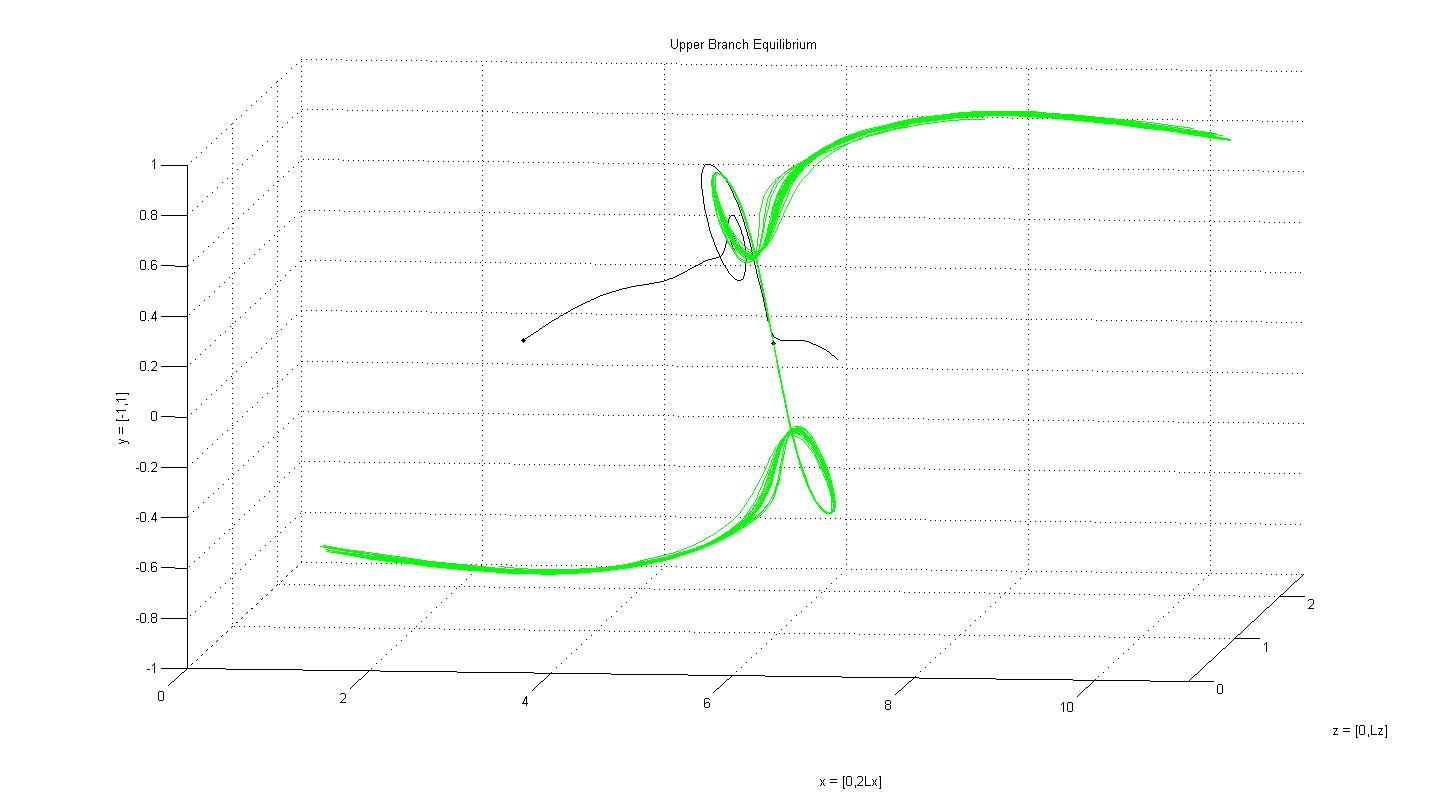
\includegraphics[width=1.3\textwidth]{almost_hetero42.jpg}
  \caption{
   Stable manifold of $\tSP{2}$ (black curve)
   and unstable manifold of $\tSP{4}$ (green surface) }
  \label{eltonFig:almost_hetero42}
 \end{figure}

Possibly heteroclinically connected pairs are $\tSP{1} \to \tSP{3}$
 and $\tSP{2} \to \tSP{4}$, and the behavior for each pair is the same except
 that one pair is shifted by $L_x/2$ from the other pair, so really
 there is only pair of points to consider and the behavior of the
 other pair will mimic the first. The pairing occurs streamwise
 rather than spanwise.  As in \refsect{sec:velgradmat},
 local stability analysis shows that $\tSP{1}$ has all real eigenvalues
with a 1D stable manifold,
and a 2D unstable manifold which is locally a plane. $\tSP{3}$
 has a 2D unstable manifold with complex eigenvalues which spiral
 out in a plane and a 1D stable manifold. Computing these manifolds
 numerically beyond the linear regime shows that there `might' exist
 \hec\ between this pair (and likewise the
 other pair $\tSP{2}$ and $\tSP{4}$). Unfortunately I do not yet see an
 analytical argument for why this should or should not exist. Since
 the pairing is between \stagp s of a qualitatively different nature
 (not just eigenvalues sign-flipped) a time
 reversal argument does not imply the connection. It is still certainly
 possible that there are other symmetries of \pCf\ which I have not
 considered that might imply a connection.

 To be more specific about ``there `might' exist \hec s,''
 refer to \reffig{eltonFig:almost_hetero24}. We see the
 stable manifold of $\tSP{4}$ (red curve) and the unstable manifold of
 $\tSP{2}$ (blue surface). The stable manifold of $\tSP{4}$ is computed by
 starting a trajectory along the stable eigenvector very close to the
 \stagp\ and integrating backwards in time.
 The unstable manifold of $\tSP{2}$ is computed by starting many
 trajectories in the plane spanned by the real and imaginary parts
 of the unstable complex eigenvectors and integrating them forward in
 time. I am using the exact sum to give the velocity field at each
 step rather than the interpolation method in order to assure
 greatest accuracy. We see that as the unstable
 manifold evolves the initial plane begins to tilt and trajectories eventually
 start to spread out along paths which appear to mimic the stable
 manifold of $\tSP{4}$. This suggests that there may in fact be a single
 trajectory originating form $\tSP{2}$ that connects exactly with $\tSP{4}$.
 Of course, because the unstable manifold is 2D it is very difficult
  to numerically find the single curve which makes this connection.
  Also, one must question the accuracy of the integration method
  once these manifolds are evolved far outside of the linear
  neighborhood.

  In the other direction, referring to \reffig{eltonFig:almost_hetero42},
  we see this time the
  stable manifold of $\tSP{2}$ (black curve)
  and the unstable manifold of $\tSP{4}$ (green
  surface). The black curve appears to "almost" connect with
  $\tSP{4}$. Again, it could be a numerical issue since close to $\tSP{4}$
  the unstable directions will cause rapid stretching of nearby
  trajectories. However since the green surface is entirely shuffled
  off in the positive $x$-direction it looks like something else may
  be happening.

   The loop-de-loop region shared by the stable and
  unstable manifolds in \reffig{eltonFig:almost_hetero42}
  suggests the possible existence of
  another pair of  \stagp s (pair because it is symmetric on the
  lower half). It looks like this point would have a pair of complex eigenvalues
  with negative real part and a single positive, real eigenvalue. To
  investigate I have created a more refined grid of velocities which
  is $144 \times 105 \times 144$. This is three times the 48 $\times$ 35
  $\times$ 48 grid in each dimension and contains about 2.2 million
  points. At each point $|\bu|^{2}$ is then calculated and at
  every point that satisfies $|\bu|^{2} < \epsilon$ for some
  arbitrarily chosen $\epsilon$, the point is plotted.
  \reffig{eltonFig:fine_usquare} shows the
  result for $\epsilon = 10^{-4}$. The blue blobs are the points which satisfy this condition
  and they have been plotted along with the same manifolds from \reffig{eltonFig:almost_hetero42}. It appears that we have isolated the
  regions with the already known \stagp s as well as the two
  regions containing the potential new ones. With a more stringent
  requirement on $\epsilon$ the point in this new region with
  smallest value for $|\bu|^{2}$ is found to be
  (see \refeq{eqn:newspNewt} for the precise value)
  \beq \label{eqn:newsp}
  \bx \simeq (2.33476, 0.40952, 0.64577) \,,\quad
  |\bu|^{2} = 2.75 \times 10^{-6}
  \eeq
  In \reffig{eltonFig:newfp} this single point (a barely visible red dot)
  is plotted along with the stable manifold
  of $\tSP{3}$. This figure looks suggestive not only that this is a
  \stagp, but there may also be a \hec\ from this point
  to $\tSP{3}$.

  Clearly the point \refeq{eqn:newsp} is not the exact \stagp\ or
  $|\bu|$ would be 0 to within machine precision. However,
  the smallest gridpoint value of $|\bu|^{2}$ in the regions
  where we \emph{know} \stagp s exist is only about $10^{-7}$, in the
  same range. As outlined in \refsect{sect:whattodo}, the next step will be to
  interpolate recursively until the exact point is found. In
  addition, no other regions appeared to within these tolerances, so
  we may have found all of the \stagp s.

\begin{center}
\begin{figure}[!h]
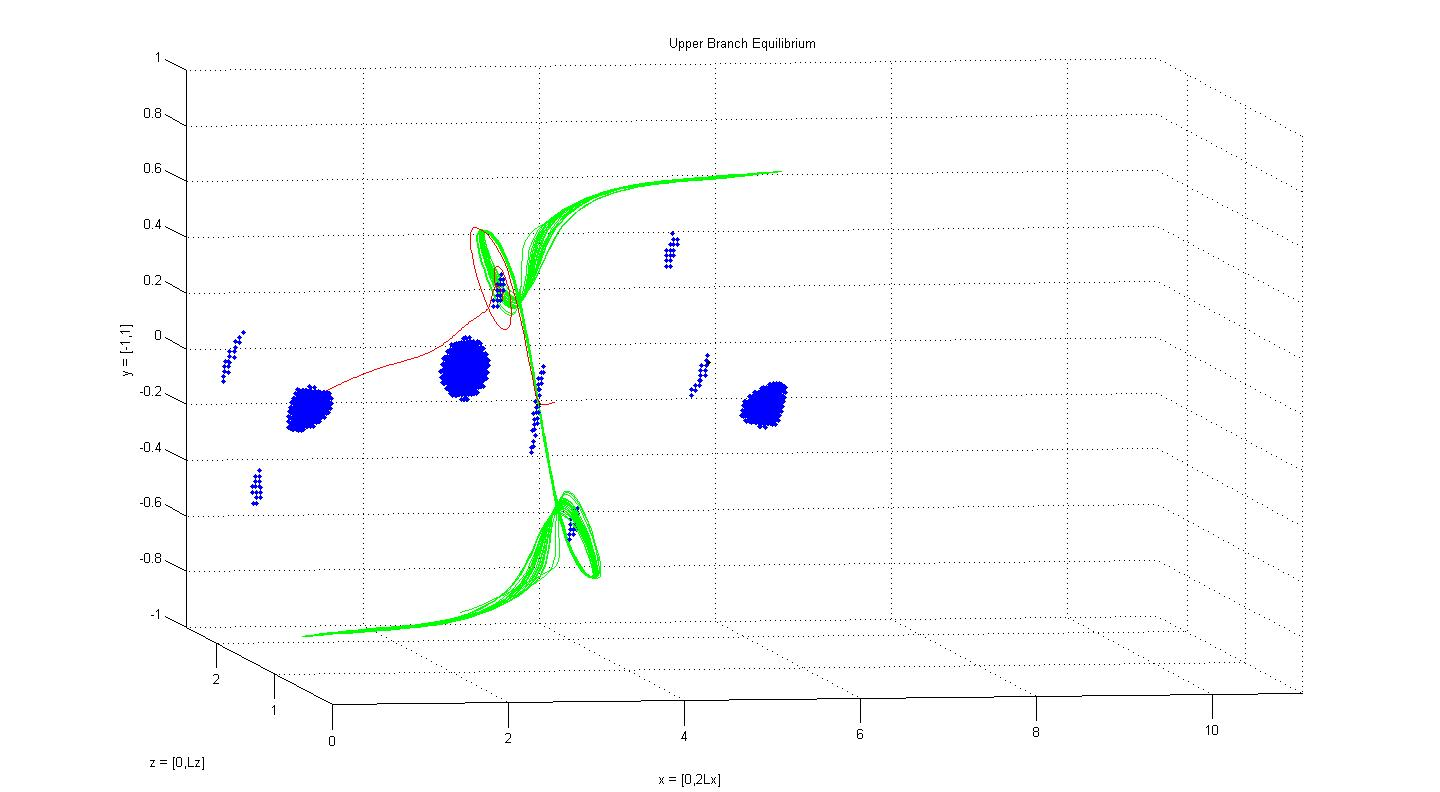
\includegraphics[width=1.3\textwidth]{fine_usquare.jpg}
  \caption{
   Blue points are where velocity squared is very near zero.
   Shown along with the stable manifold
   of $\tSP{3}$ and the unstable manifold of $\tSP{1}$.
          }
  \label{eltonFig:fine_usquare}
 \end{figure}
\end{center}

\begin{center}
\begin{figure}[!h]
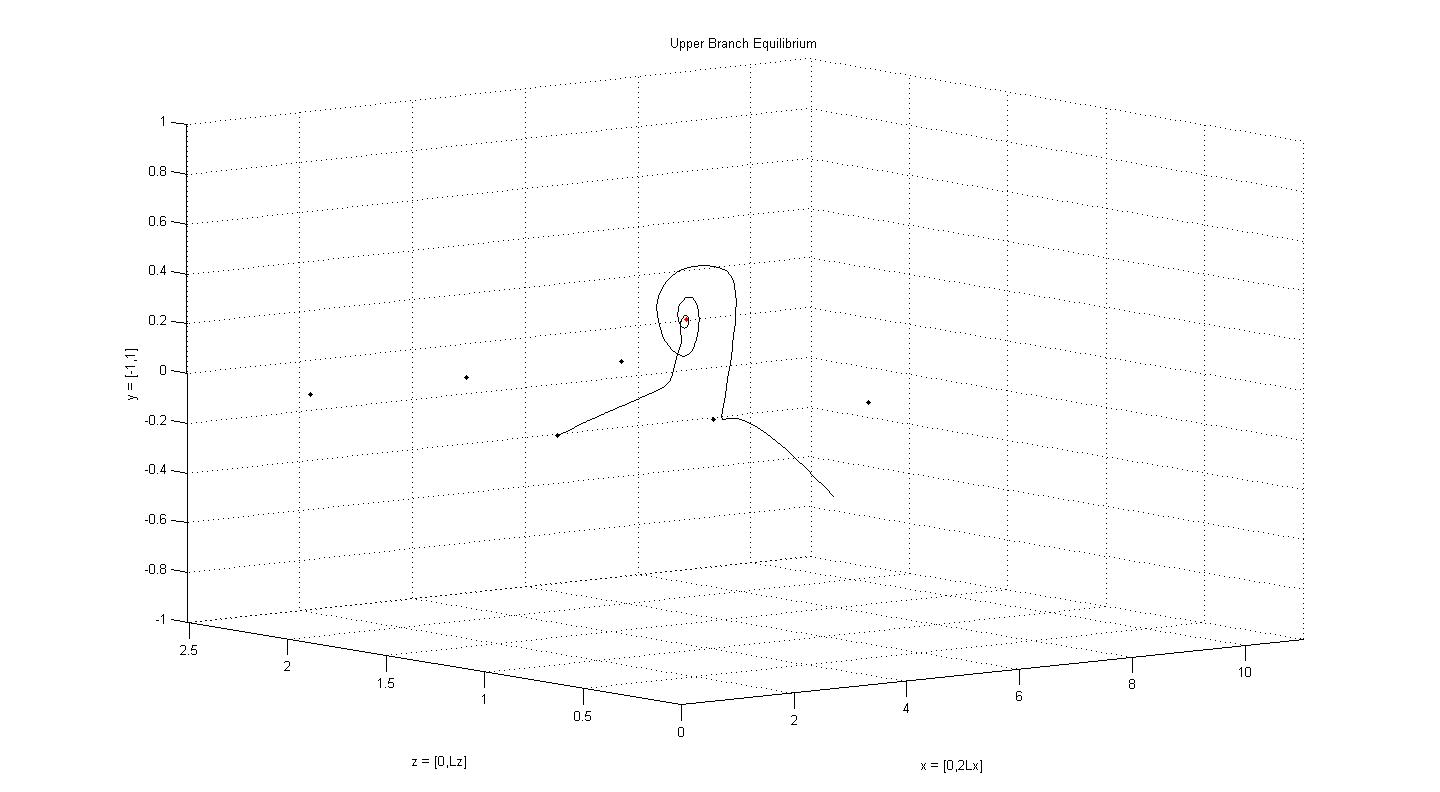
\includegraphics[width=1.3\textwidth]{newfp.jpg}
  \caption{
   Shows a single red point within the tangled region of the stable manifold of $\tSP{3}$.
   This point has a velocity close to zero and is expected to be very near a \stagp.
          }
  \label{eltonFig:newfp}
 \end{figure}
\end{center}


\noindent
[{\bf PC May 26, 2008}: moved ``local Reynolds number \Reynolds(\bx)'' musings to
\refsect{sec:Rey}]

\section{\Velgradmat\ and its eigenvalues}
\label{sec:velgradmat}

\noindent {\bf JRE May 15, 2008}: For a perturbation $\delta$\bx\
the change in the velocity field is given by $\delta\bu = \Mvar
\delta\bx$ where $\Mvar$ is the nine component \velgradmat\ defined
by $\Mvar_{ij}=\frac{\partial u_{i}}{\partial x_{j}}$. Since \bu\ is
given by \refeq{eqn:spectralsum}, it is a relatively simple
extension of this formula to evaluate these partials. To find
$\partial\bu/\partial y$, one needs to use the relation
$\frac{\partial}{\partial y}T_{n}(y) = n U_{n-1}(y)$ where $T_{n}$
is the $n$th Chebyshev polynomial of the first kind and $U_{n}$ is
the $n$th Chebyshev polynomial of the second kind. Everything else
is straightforward.


The eigenvalues of $\Mvar$, evaluated at a \stagp\ , give local stability
and reveal the qualitative nature of the motions nearby the \stagp.
For the four \stagp s we have so far the eigenvalues, eigenvectors,
and velocity gradients matrices are as follows. \\

$\xSP{1}=(L_x/2,0,L_z/4)$: There are 3 real eigenvalues, two positive and one
negative.
\begin{align}
&\eigExp[1] = -0.4652099 \,,\quad
\jEigvec[1] =
\begin{pmatrix}
             {0.9844417} \cr
             {0.1743315} \cr
             {0.0219779} \cr
   \end{pmatrix} \\
    &\eigExp[2] = 0.4008961 \,,\quad \jEigvec[2] =
\begin{pmatrix}
             {0.5704000} \cr
             {-0.7666749} \cr
             {0.2947091} \cr
   \end{pmatrix} \\
    &\eigExp[3] = 0.0643139 \,,\quad \jEigvec[3] =
\begin{pmatrix}
             {0.4082166} \cr
             {0.7525949} \cr
             {0.5166819} \cr
   \end{pmatrix} \end{align}
   The \velgradmat\ is
\beq
   \Mvar =
   \begin{pmatrix}
   {-0.4305385} &  {-0.3002042} &{0.8282447} \cr
   {-0.1221356} &   {0.2456107} & {-0.1675796} \cr
   {0.0001651}  &   {-0.0828951}  & {0.1849278} \cr
            \end{pmatrix}
\eeq
    The point is a saddle; It has 1 stable dimension and a 2D plane
    of instability spanned by $\mathbf{v_{2}}$ and $\mathbf{v_{3}}$.
    The eigenvalues sum to 0, as is required by volume conservation
    (If you add the values shown here to check this by hand, note that I have
    rounded them. When they are added on the computer it comes out
    to be 0 within machine precision, $\sim10^{-16}$).
     The \stagp\ at
    $(0,0,3L_z/4)$ has the same eigenvalues as this point. It's
    eigenvectors and \velgradmat\ differ by a minus sign
    in the third component (except for $\Mvar_{33}$ where the two minuses
    cancel). \\

$\xSP{2}=(L_x/2,0,3L_z/4)$: There is one real, negative eigenvalue and a complex
pair with positive real part.
    \PC{rewrite eigenvectors in their real form}
\begin{align}
&\eigExp[1] = -0.0352362 \,,\quad \jEigvec[1] =
\begin{pmatrix}
             {-0.9452459} \cr
             {-0.1893368} \cr
             {-0.2658228} \cr
   \end{pmatrix}
   \\
&\eigRe[2] \pm i\,\eigIm[2] = 0.0176181 \pm i\,0.0862176
   \\
&\jEigvec[2] =
\begin{pmatrix}
             {0.3737950 + 0.0544113i} \cr
             {0.2098940 - 0.4925773i} \cr
             {0.7554000} \cr
   \end{pmatrix}
\,,\quad
\jEigvec[3] =
\begin{pmatrix}
             {0.3737950 - 0.0544113i} \cr
             {0.2098940 + 0.4925773i} \cr
             {0.7554000} \cr
   \end{pmatrix}
\nnu\,.
\end{align}
The \velgradmat\ is \beq
   \Mvar =
   \begin{pmatrix}
   {-0.0316935} & {-0.0708737} &  {0.0378835} \cr
  {-0.0250579} & {-0.0218884} &  {0.0795969} \cr
   {0.0014742} & {-0.1320575} &  {0.0535818} \cr
   \end{pmatrix}
                    \eeq

    This \stagp\ spirals out in a plane given by the complex pair of
    eigenvectors. It is stable in one dimension that is dominantly
    along the $x$ direction. As with the first pair of points, the
    \stagp\ at $(0,0,L_z/4)$ has the same eigenvalues and again, the
    \velgradmat\ is the same except for sign changes in
    the third component. This follows from the symmetry arguments.
    We now want to understand the connections between the manifolds.


\section{Rough sketch of topics}

\noindent {\bf JRE May 12, 2008}: After using the sum formula
discussed in \refsect{sec:streaml} to compute \textbf{u} at every
point along a trajectory, I have switched to an interpolation method
because of run-time issues. Using the previous method, I create an
arbitrarily fine set of gridpoint values for $\textbf{u}$ and then
use a bilinear(trilinear?) interpolation method. (\textbf{Note:} To
the eye it looks like this works pretty well but I need to look at
the numerical values more closely and check the accuracy of the
interpolation. How fine should I make the grid? Always need to be
careful about approximations in the chaotic regime).

The starting point is clear because we already have four \stagp s
predicted from translational symmetries of \pCf. Starting a small
sphere of initial conditions around the \stagp s and evolving them
forward and backward in time gives a good estimate of the stable and
unstable manifolds. Results are shown in
\reffig{eltonFig:manifolds_both}. From these we begin to get a feel for
the dynamics. Also, I can create movies to show the evolution of a
ball of little ink droplets moving through the fluid, but I need to
get these from .mat format to mp3's before I can post them anywhere.
Being able to visualize the stretching and folding of these material
lines and surfaces will be a key point.

This rough visualization of the manifolds is nice, but much better
can be done. Since we have a sum formula for computing velocities at
any point, by differentiating under the sum it should be a simple
matter to compute the $[3\!\times\! 3]$ {\velgradmat}
at any point. Eigenvalues / eigenvectors of this matrix will
give linear stability and allow for exact computation of the stable
and unstable manifolds. There are several expectations/predictions
of what we'll find: (1) Will have one real eigenvalue and one
complex pair. Judging from \reffig{eltonFig:manifolds_both} I'm
not sure about this one yet. It certainly looks true for the
black/blue \stagp, but for the other one it seems unclear what is
going on. The stretching is strong around this point so it may be
that the plane is quickly dominated in one direction and appears to
collapse to a line, or it may be that all the eigenvalues are real.
(Prepare to edit this section as soon as I have the answer.) (2) The
eigenvalues for the two points should be the same but with signs
reversed resulting from translational symmetry, and this amounts to
time reversal invariance. I'm a little confused on this one, I would
appreciate a comment from anyone with an explanation. (3) There is a
\hec\ between the \stagp s. Will find out soon,
this would be great for using chaos. Apparently the time reversal
would force this connection.

After exhausting these four points we will want to find other
stagnation points, either by using other symmetries or numerically.
The numerical task would involve computing $u^{2}$ all along the
grid and spotting regions where it is below a given threshold. Then
using an interpolation in the small regions the \stagp s can be
pinned down. The same eval/evec stable/unstable manifold analysis
can then be done for any other \stagp.

The long term goal after all of this is of course to compute mixing
and diffusion properties; Lyapunov exponents, material stretching,
striation thickness, time to mix etc... Most investigations like
this tend to be in two dimensional closed systems, but if we find we
have good Lagrangian chaos, there is no reason not to do it here.

\begin{figure}[!h]
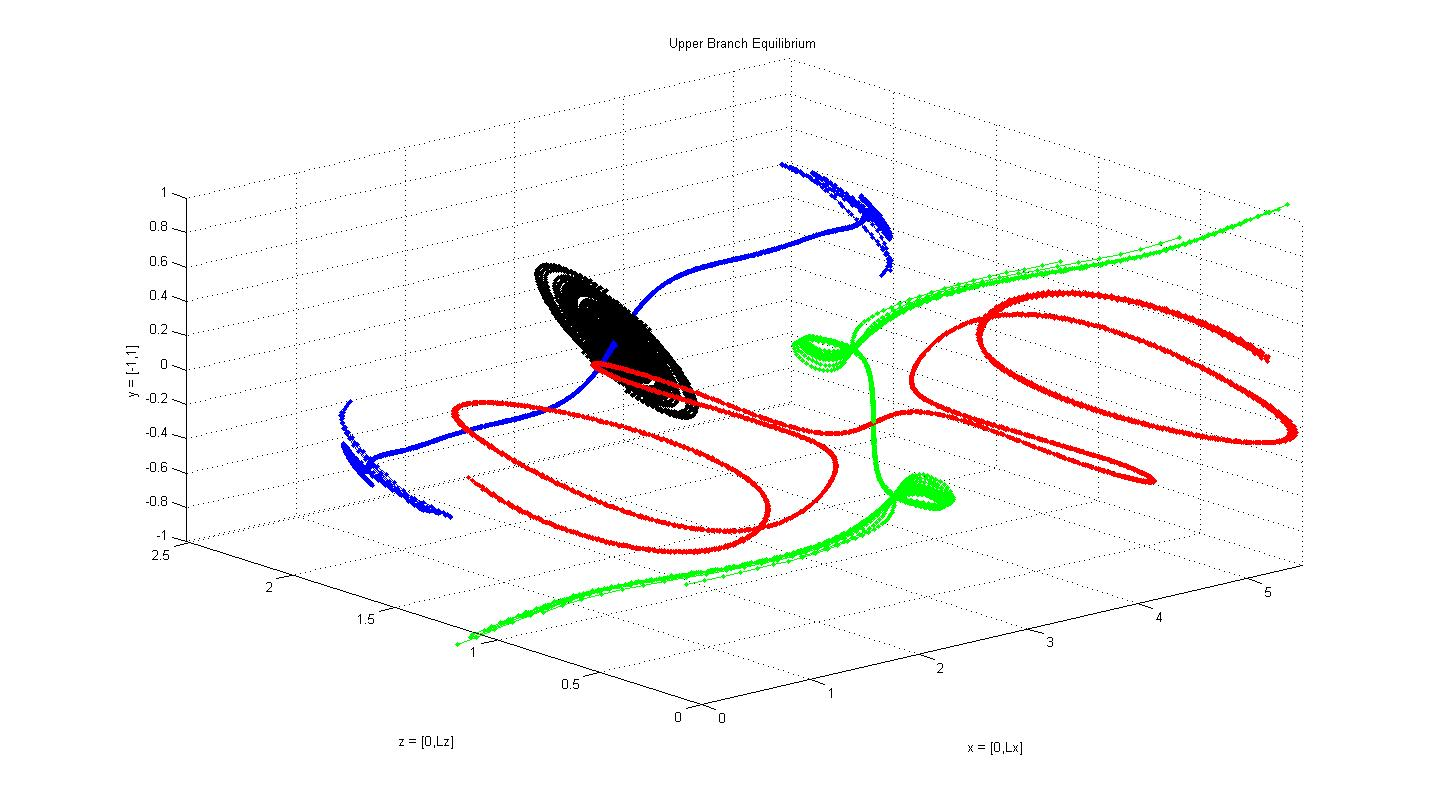
\includegraphics[width=1.3\textwidth]{manifolds_both.jpg}
  \caption{
   Stable and unstable manifolds of the \stagp s
   $\xSP{1} = (L_x/2,0,L_z/4)$ and
   $\xSP{2} = (L_x/2,0,3L_z/4)$. Black and green are unstable.
   }
  \label{eltonFig:manifolds_both}
 \end{figure}


\section{Notes on mixing}

General discussion and notes about mixing in fluids, largely taken
from the book by J.M. Ottino (see reading assignments). \\

Coming soon.


\section{Mixing and \stagp s for \tUB}

\noindent {\bf JRE  April 29, 2008}: Our starting point is the data
set computed by Gibson\rf{channelflowDat} of the Nagata/Walleffe
``upper branch'' \eqv\ \tUB, for $\Reynolds = 400$, the
Waleffe\rf{W03} small-aspect cell \beq \bNarrow =  [L_x,2,L_z]
         = \; [2\pi/1.14,2,4\pi/5]
         = [5.511566,2,2.513274]
%         = [5.51156605892946182182,2,2.51327412287183459075]
\,.
\label{cellW03}
\eeq

To begin looking at the evolution of Lagrangian tracers in the
\eqv\ \tUB, I have first integrated a grid of initial points. The grid
is chosen to lie in the $[y,z]$ plane, centered at $x = L_x/2$. The initial
points are equally spaced, and offset by one position from the edge
of the box. If the number of points is chosen to be one less than a
multiple of 4, there will be points starting at $\xSP{1}=(L_x/2,0,L_z/4)$ and
$\xSP{2}=(L_x/2,0,3L_z/4)$. Similarly, if we make the grid be centered at x = 0,
we will have points starting at $(0,0,L_z/4)$ and $(0,0,3L_z/4)$. The
trajectories are run for 15 seconds, and the results of this are
shown in \reffig{eltonFig:UBs}\;(a) and \reffig{eltonFig:UBw}\;(a).
\JRE{
  The figures need some editing. It's almost impossible to read
  the axis labels. Also, they won't go where I want them to!
   }

Invariance under the symmetry group $\bf S$, explained by JH in
\refsect{JHsec:4/28}, implies the existence of 4 \stagp s
\refeq{s3lagrange}.
%\bea
%  \xSP{1} &=& (L_x/2,0,L_z/4) \continue
%  \xSP{2} &=& (L_x/2,0,3L_z/4) \continue
%  \xSP{3} &=& (0,0,L_z/4) \label{s3lagrange} \\
%  \xSP{4} &=& (0,0,3L_z/4) \nnu
% \,.
%\eea
In \reffig{eltonFig:UBs}(b) and \reffig{eltonFig:UBw}(b) the figures
from part (a) have been rotated to almost a y-z projection in order
to reveal these \stagp s. The behavior of trajectories near these
fixed points seems to reveal "what kind" of fixed points they are.
The point at $3L_z/4$ in \reffig{eltonFig:UBs}(b) appears to be an
unstable out-spiral, whereas the point at $L_z/4$ is probably hyperbolic.
There is also some other interesting behavior going on near the
point at $L_z/4$. The next step is probably to look at eigenvalues and
stable/unstable manifold of these \stagp s.



    {\bf JFG April 30, 2008} The plots of tracers and the derivation of
\stagp s from symmetries are very interesting.

I see from \reffig{eltonFig:UBw} and \reffig{eltonFig:UBs} that
you're plotting tracers for the difference from laminar flow. (You
can see $u \rightarrow 0$ as $y \rightarrow \pm 1$.) I don't know if
this is intentional. If it's not, sorry, we haven't been
sufficiently clear on the definitions of data we gave you. We
usually work with $\bu$ defined as the difference from laminar flow,
so that the total velocity field $\bu_\text{tot} = \bu + y {\bf
\hat{x}}$. So you might want to add the laminar flow  $y {\bf
\hat{x}}$ on to $\bu$ before computing tracers. That'll produce $u
\rightarrow \pm 1$ as $y \rightarrow \pm 1$. The \stagp s are all
at $y=0$, so they will not change.

{\bf JRE May 02, 2008} No, that was not intentional. I had forgotten
that the velocity fields were computed \emph{from} laminar. From now
on all plots are of $\bu_\text{tot}$.


\begin{center}
\begin{figure}[!h]
(a)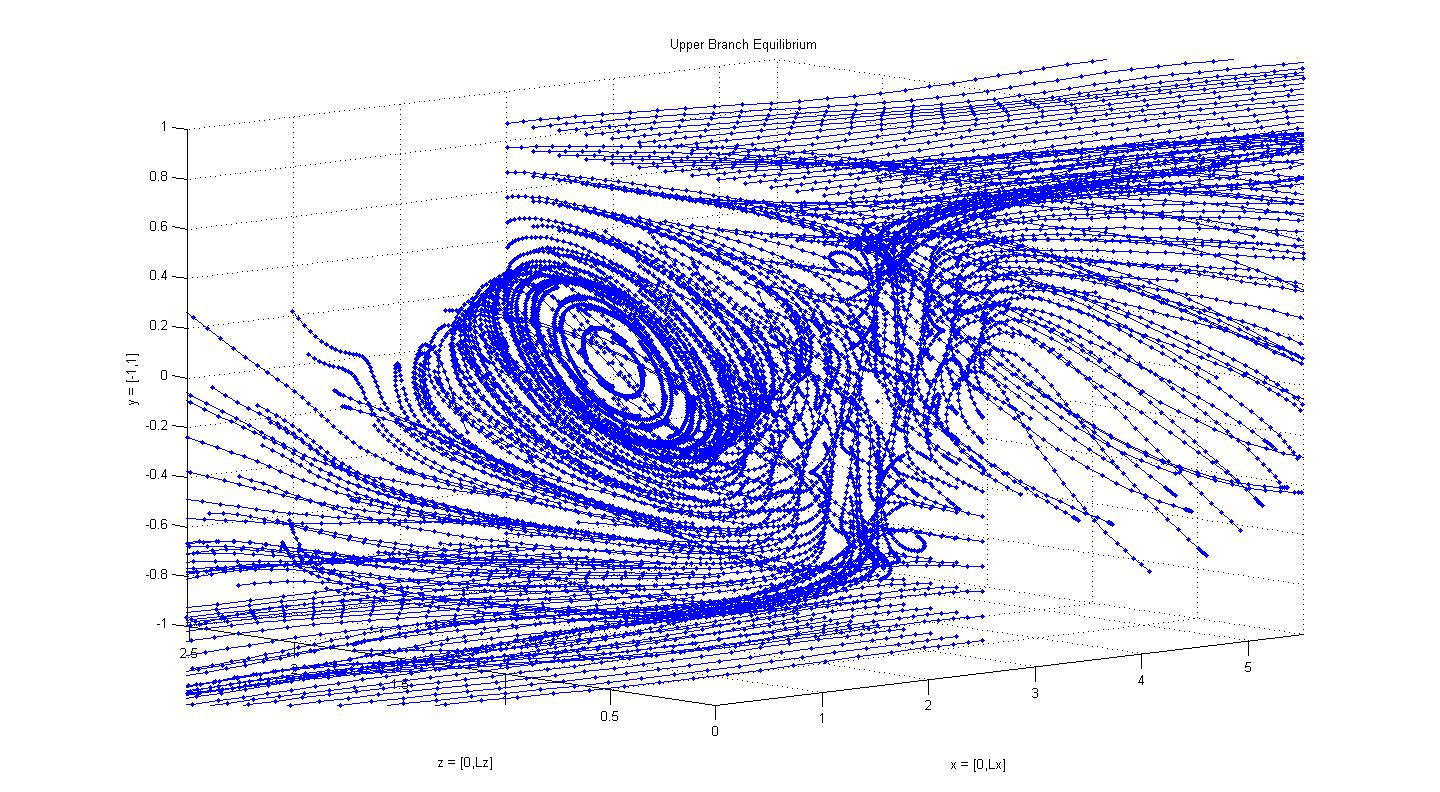
\includegraphics[width=1.3\textwidth ]{fig_UB1.jpg}
(b)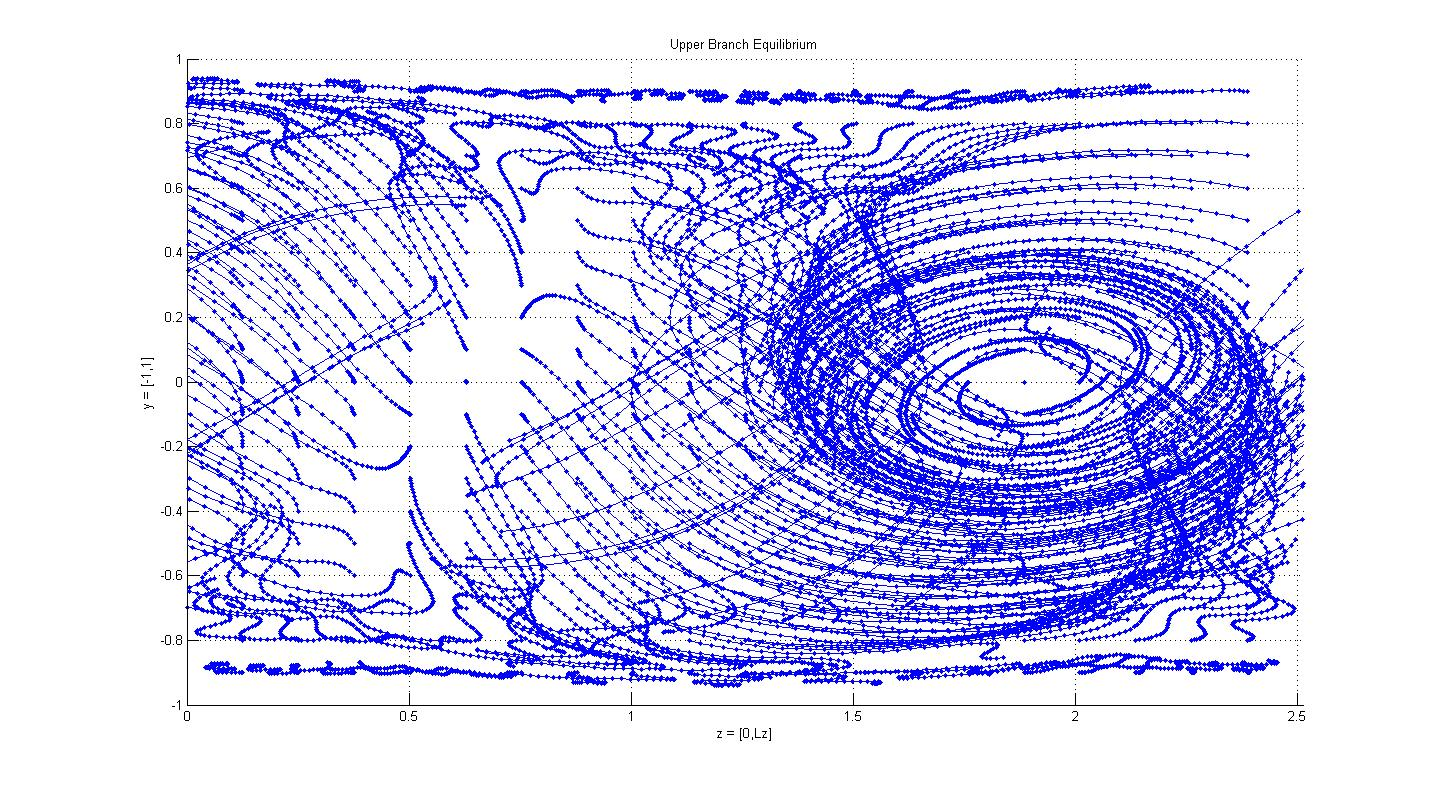
\includegraphics[width=1.3\textwidth]{fig_UB1eq.jpg}
  \caption{
  (a) {Grid of $19 \times 19$  initial points in the $[y,z]$ plane,
centered at $x = L_x/2$; integrated for 15 time units.}
    (b) { Rotated to show the 2 \stagp s}.
      }
  \label{eltonFig:UBs}
 \end{figure}

 \begin{figure}[!h]
(a)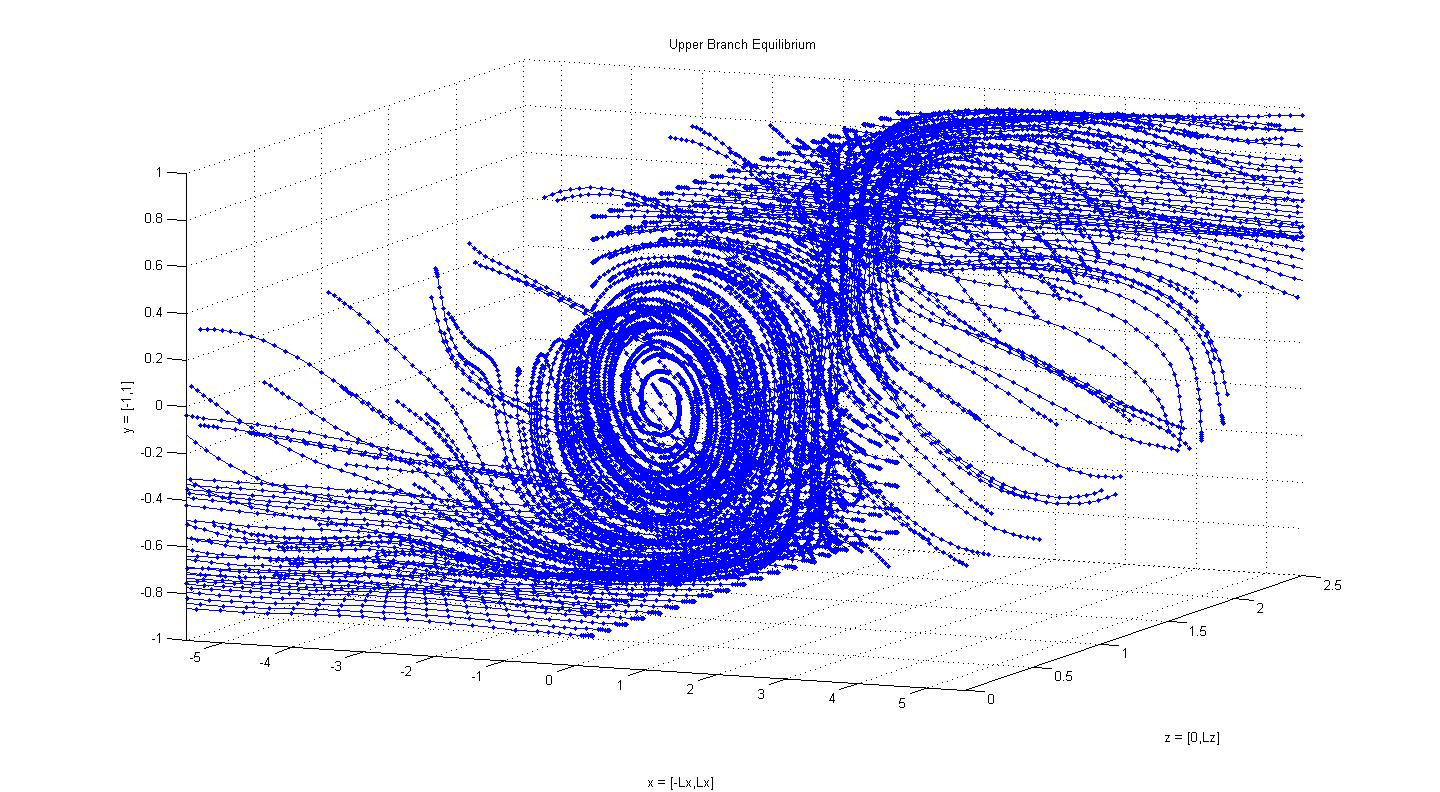
\includegraphics[width=1.3\textwidth]{fig_UB2.jpg}
(b)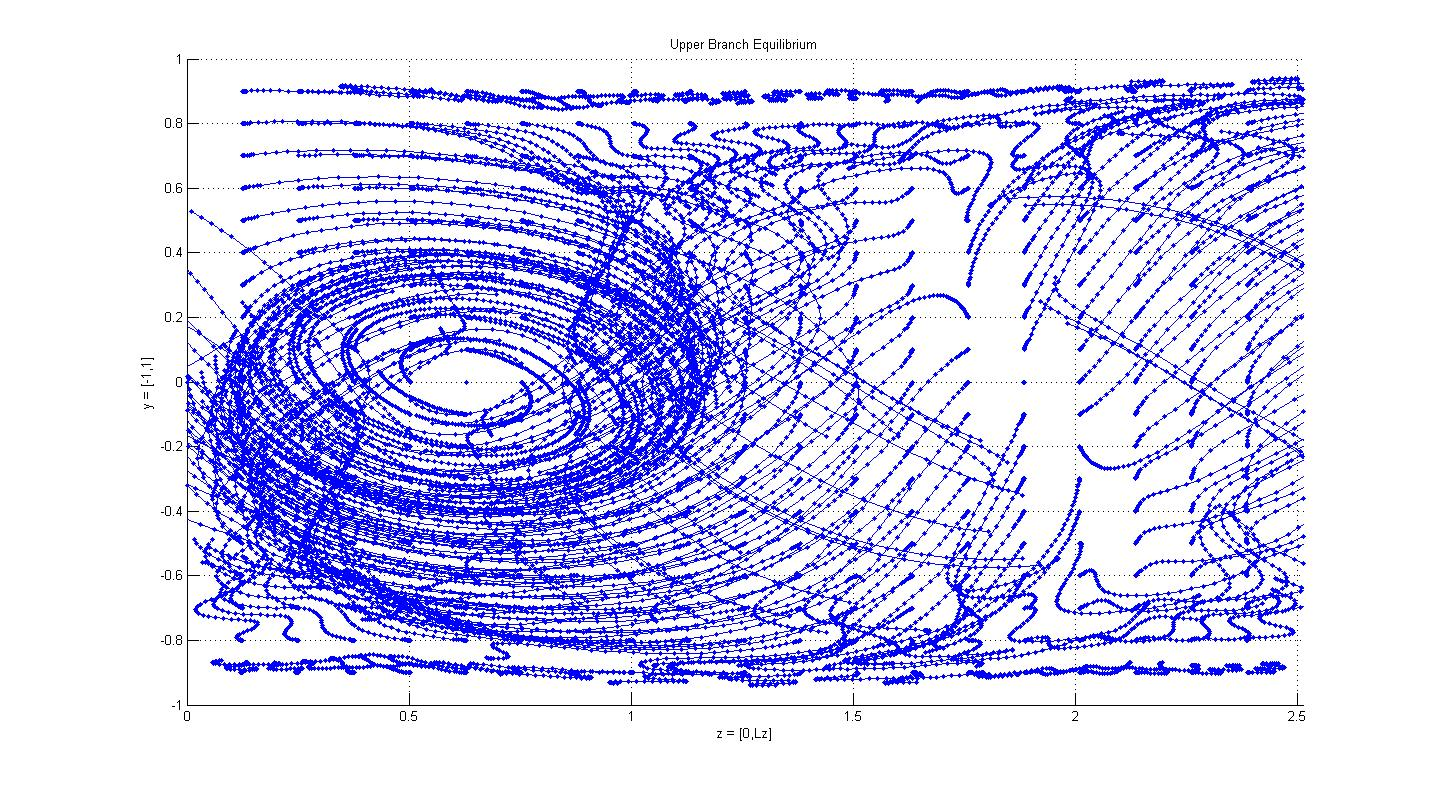
\includegraphics[width=1.3\textwidth]{fig_UB2eq.jpg}
  \caption{
  (a) {Grid of $19 \times 19$ initial points in the $[y,z]$ plane,
centered at $x = 0$; integrated for 15 time units.}
  (b) { Rotated to show the other 2 \stagp s}.
         }
  \label{eltonFig:UBw}
 \end{figure}
\end{center}



\section{Symmetry and \stagp s}
\label{JHsec:4/28}

\PCf\ is invariant under two reflections $\sigma_1,\sigma_2$ and a
continuous two-parameter group of translations $\tau(\shift_x, \shift_z)$:
\begin{align}
\sigma_1 \, [u,v,w](x,y,z) &= [u, v,-w](x,y,-z) \nnu \\
\sigma_2 \, [u,v,w](x,y,z) &= [-u,-v,w](-x,-y,z)  \label{reflSfit1}\\
\tau(\shift_x, \shift_z)[u,v,w](x,y,z) &= [u,v,w](x+\shift_x,y,z+\shift_z) \nnu\,.
\end{align}
The \NSe s and boundary conditions are invariant for any symmetry $s$
in the group generated by these elements:
$\partial (s \bu) / \partial t = s (\partial \bu / \partial t)$.

The plane Couette symmetries can be interpreted geometrically in the space of
fluid velocity fields. Let $\bbU$ be the space of
square-integrable, real-valued velocity fields that satisfy the kinematic
conditions of \pCf:
\begin{align}
 \bbU  &= \{\bu \in L^2(\Omega) \; | \; \grad \cdot \bu = 0,
               \; \bu(x, \pm 1, z) = 0, \notag  \\
         &\phantom{=} {} \qquad \qquad \qquad \; \; %\text{and }
          \bu(x, y, z) = \bu(x+L_x, y, z) = \bu(x, y, z + L_z)\}  \,.
\end{align} \JRE{Shouldn't we say $\mathbf{u}= \pm 1$ at the walls for consistency?}
The continuous symmetry $\tau(\shift_x, \shift_z)$ maps each state
$\bu \in \bbU$ to a $2d$ torus of states with identical dynamic
behavior. This torus in turn is mapped to four equivalent tori by
the subgroup $\{1,\sigma_1,\sigma_2, \sigma_1 \sigma_2\}$. In
general a given state in $\bbU$ has four $2d$ tori of dynamically
equivalent states.

Most of the Eulerian \eqva\ that we know of so far
are invariant under the `shift-reflect' symmetry
$s_1 = \tau(L_x/2,0) \, \sigma_1$ and the `shift-rotate' symmetry
$s_2 = \tau(L_x/2,L_z/2) \, \sigma_2$.  These symmetries form a subgroup
$S = \{1, s_1, s_2, s_3\}$, $s_3 = s_1 s_2$, which is isomorphic to
the Abelian dihedral group $D_2$. The group acts on velocity fields
as:
\begin{align}
s_1 \, [u, v, w](x,y,z) &= [u, v, -w](x+L_x/2,\, y,\, -z) \nnu \\
s_2 \, [u, v, w](x,y,z) &= [-u, -v, w](-x+L_x/2,\,-y,\,z+L_z/2) \label{shiftRot} \\
s_3 \, [u, v, w](x,y,z) &= [-u,-v,-w](-x,\, -y,\, -z+L_z/2) \nnu \,.
\end{align}

Consider next the subgroup $S_3 = \{1,s_3\} \subset S$ (isomorphic to
dihedral group $D_1$). The $s_3$ operation flips both the streamwise
$x$ and the spanwise $z$, thus eliminating invariance under both $x$
and $z$ continuous translations. \PC{do we need this in this paper?:
\\ ``$s_3 \bu = \bu$ implies $[u,v,w](x,y,z) =
[-u,-v,-w](-x,-y,-z+L_z/2)$, which requires $\bu = 0$ at four points
$(x,y,z) = (0,0,L_z/4); (0,0,3L_z/4); (L_x/2,0,L_z/4);
(L_x/2,0,3L_z/4)$. '' }


Let $\bbU$ be the space of square-integrable, real-valued velocity
fields that satisfy the kinematic conditions of \pCf:
\begin{align}
 \bbU  &= \{\bu \in L^2(\bCell) \; | \; \grad \cdot \bu = 0,
               \; \bu(x, \pm 1, z) = 0, \notag \\
         &\phantom{=} {} \qquad \qquad \qquad \; \; %\text{and }
          \bu(x, y, z) = \bu(x+L_x, y, z) = \bu(x, y, z + L_z)\}
\,.
\end{align}
We denote the $S$-invariant subspace of states invariant under
symmetries \refeq{shiftRot} by
\begin{align}
\bbUsymm  &= \{\bu \in \bbU  \: | \;
              s_j \bu = \bu\,, \;\;  s_j \in S \}
              % \bu = \frac{1}{4} (1 + s_1 + s_2 + s_3)\,\bu \}
\,,
\label{symmSubspU}
\end{align}
and the $S_3$-invariant subspace by
\begin{align}
\bbUthree  &= \{\bu \in \bbU  \: | \;
              s_3 \bu = \bu\,, \;\; % s_3 \in S_3\,, \;\;
              s_1 \bu \neq \bu\,, \;\;  s_2 \bu \neq \bu
               \}
\,,
\label{symmUthree}
\end{align}
where $ \bbUsymm \subset \bbUthree \subset \bbU$.
%
$\bbUsymm$ and  $\bbUthree$ are flow-invariant subspaces: states initiated
in either remain within it under the Navier-Stokes dynamics.
%     \PC{recheck this claim, please}

Idempotency of $s_3$ leads to projection operators
\beq
{\PP}_+ =
   \frac{1}{2} (\matId + s_3) \, ,\qquad
{\PP}_- =
   \frac{1}{2} (\matId - s_3) \,.
\ee{S3project}

Translations of half the cell length in the spanwise and/or streamwise
directions commute with $S$. These operators generate a discrete
subgroup of the continuous translational symmetry group $SO(2) \times
SO(2)$ :
\beq
T = \{e,\tau_x,\tau_z,\tau_{xz}\}
    \,,\qquad
    \tau_x = \tau(L_x/2,0)
    \,,\;
    \tau_z = \tau(0,L_z/2)
    \,,\;
    \tau_{xz} = \tau_x \tau_z
\,.
\ee{tauD2}
Since the action of $T$ commutes with that of $S$,
% the $T$-group orbit of each velocity field $\bu \in \bbUsymm$
% is also contained in $\bbUsymm$.
% More explicitly:
the three half-cell translations $\tau_x \bu, \, \tau_z \bu,$ and
$\tau_{xz} \bu$ of $\bu \in \bbUsymm$ are also in $\bbUsymm$.
Similarly, $\tau_{xz}$ commutes with $S_3$, so $S_3$-invariant
solutions appear in eight copies.
\PC{
    incorporate halcrow blog JFG comment for the the $S_3$-invariant claim,
    please: if you agree, comment out this footnote.
    }




\noindent {\bf JH  April 28, 2008}:
From the form of $s_3$, we can see that any Eulerian $\eqv$ that
is invariant under has 4 Lagrangian \stagp s
which satisfy the condition:
\begin{equation}
 (x,y,z) = (-x, -y, -z+L_z / 2) \label{shiftRot_eqva}
\end{equation}
There are 4 points which satisfy this constraint:
\bea
  \xSP{1} &=& (L_x/2,0,L_z/4) \continue
  \xSP{2} &=& (L_x/2,0,3L_z/4) \continue
  \xSP{3} &=& (0,0,L_z/4) \label{s3lagrange} \\
  \xSP{4} &=& (0,0,3L_z/4) \nnu
 \,.
\eea
Due to the periodic boundary conditions
 $(L_x,0,L_z/4)=\tSP{3}$ and $(L_x,0,3L_z/4)=\tSP{4}$.
Also of note is the fact that there can exist no $s_3$-invariant \reqva, since
$s_3$ operation flips both the $x$ and $z$ axes.


\noindent {\bf PC  May 25, 2008}: moved \refsect{sec:streaml}
to \refchap{chap:channelflow}.



\section{Notational conventions}

\noindent{\bf Predrag, May 12, 2008:}
In Lagrangian mixing we need to distinguish between
$3D$ physical fluid flow (for a given invariant solution)
and the dynamical $\infty$-dimensional \statesp\ flow.

We distinguish the two by using physically motivated nomenclature
for $3D$ physical fluid flow: We shall refer to the $3D$ point
\bx\ for which
$\bu(\xeq{})=0$
as the {\em \stagp} \xeq{}, and
the moving point \bx(t) for which
$\bu(\xtw{})=0$,
$\xtw{} - {\bf c} t = \bx_{\text{\tiny tw}}(0)$
as the {\em \relstagp} \xtw{}.

%We distinguish the two by using physically motivated nomenclature
%for $3D$ physical fluid flow: We shall refer to the $3D$ point \bx\
%for which $\bu(\xeq{})=0$ as a {\em \stagp} \xeq{}, and the moving
%point \bx(t) for which $\bu(\xtw{})=0$, $\xtw{} - {\bf c} t =
%\bx_{\text{\tiny tw}}(0)$ as the {\em \relstagp} \xtw{}.


(to be continued:
 \velgradmat% velocity gradients matrix
, \etc.)

\noindent{\bf Predrag to Jonathan, Oct 13, 2007:}
\Reqva\ are not periodic, they are stationary in the
velocity ${\bf c}$ co-moving frame. Rather than using ``period of $T$"
description (such as ``$x$ traveling with a period of $T=169.62747092815$"),
state that \REQV{\pm}{1} has velocity
$c_x = L_x/T $?

\section{Integrating velocity fields}
\label{ssect:IntVel}

\noindent{\bf Predrag Nov 2, 2007 to
    \HREF{http://www-msnm.univ-mrs.fr/schneider.htm}{Kai Schneider}:}\\
John Elton is planning to use some of
the exact {\pCf} solutions computed by Waleffe, Viswanath,
Gibson and Halcrow (data
sets are on \HREF{http://channelfow.org}{channelfow.org})
and study Lagrangian tracer trajectories for such solutions. Marie Farge
(farge@lmd.ens.fr) tells me that many people do this
inaccurately, but you know how to do it right. Let us know what we
should read not to waste time
on not doing it right?

\noindent{\bf Kai Schneider:} (kschneid@cmi.univ-mrs.fr)\\
Concerning Lagrangian particles:
 it is important to use the right techniques for time integration
 and for interpolation of the velocity (and acceleration)
 for computing them accurately.

For time integration we are using a second order
Runge-Kutta scheme and for space interpolation a bicubic (in 2d) scheme.

There is a nice recent paper by Homann, Dreher and Grauer\rf{homann-2007}
and an older one by P.K. Yeung and Pope\rf{YeuPop06}
(you have the specialist on that just next 10 buildings away).


\section{Passive scalar advection?}

\noindent {\bf PC Nov 2, 2007}:
The
other thing we might try is passive scalar transport using these
velocity fields (but that I really have barely started thinking
about).

Very sketchy:

Given a velocity field, densities (passive scalars?)
are advected by th  %(generalized)
{\em Fokker-Planck equation}
\index{Fokker-Planck equation}
\beq
\partial_t \msr + \partial_i(\msr v_i)=\DiffC \, \partial^2 \msr.
\ee{FokkPlanck}
%  (The symbol nabla $\nabla$ denotes the divergence when it acts on vectors
%  and the gradient, when it acts on scalars.)
The left hand side,
$d\msr/dt = \partial_t \msr + \partial \cdot (\msr v) $,
is deterministic, with
the
{continuity equation} % \refeq{Cont}
recovered in the weak noise limit $\DiffC\rightarrow 0$.
The right hand side describes the diffusive transport
in or out of the material particle volume.
If the density is lower than in
the immediate neighborhood, the local curvature is
positive, $\partial^2 \msr > 0$, and the density grows.
Conversely, for negative curvature
% (top of a hill)
diffusion lowers the
local density, thus smoothing the variability of $\msr$.

Not sure that this is the thing we want to investigate, and sure do not know
how to think about the diffusive part $\DiffC \, \partial^2 \msr$. Easier to
try playing with tracer particles first...

\noindent
{\bf JFG 2008-04-29:} If we want to do this, it would not be hard to integrate
the Fokker-Planck equation using channelflow, at least with an explicit time-stepping
method. Express the probability density as a 1d FlowField, compute the $\partial_i(\msr v_i)$
and $\DiffC \, \partial^2 \msr$ terms using differential operators, and add them together
using Adams-Bashforth, Runge-Kutta, or similar formulae to get an update equation for the
density. It would not take many lines of code.
